\documentclass[12pt]{article}
\usepackage[utf8]{inputenc}
\usepackage[english,main=dutch]{babel}

\usepackage{systeme}
\usepackage{amsthm}
\usepackage{amsfonts}
\usepackage{amsmath}
\usepackage{amssymb}
\usepackage{graphicx}
\usepackage{subcaption}
\usepackage{float}
\usepackage[left=3cm,right=2cm,top=2.5cm,bottom=2.5cm]{geometry}
\usepackage[export]{adjustbox}
\usepackage[nottoc]{tocbibind}
\usepackage{tikz}

\DeclareMathOperator{\sn}{sn}
\DeclareMathOperator{\cn}{cn}
\DeclareMathOperator{\dn}{dn}

\newtheorem{defn}{Definitie}
\newtheorem{lem}[defn]{Lemma}
\newtheorem{stl}[defn]{Stelling}
\newtheorem{opm}[defn]{Opmerking}
\newtheorem{vbn}[defn]{Voorbeeld}
\newtheorem{nta}[defn]{Notatie}

\renewcommand{\maketitle}{
\begin{titlepage}
\begin{figure}
    \centering
    \begin{subfigure}{0.49\textwidth}
    \includegraphics[width=0.8\textwidth]{logo_ugent.png}
    \end{subfigure}
    \begin{subfigure}{0.49\textwidth}
    \includegraphics[width=\textwidth,right]{logo_faculteit.png}
    \end{subfigure}
\end{figure}
    \textbf{}
    
    \vspace{2cm}
    \centering
    \Huge
    \textbf{Multiparametrische exponentieel gefitte Runge-Kutta-methodes}
    
    \vspace{0.5cm}
    \Large
    \textbf{Robin Keppens}
    
    \vspace{0.5cm}
    \large
    \textbf{Promotor: Prof. dr. Marnix Van Daele}
    
    \vspace{0.5cm}
    \small
    \textbf{Vakgroep toegepaste wiskunde, informatica en statistiek}
    
    \vspace{7cm}
    \small
    Masterproef ingediend tot het behalen van de academische graad van master in de wiskunde
    
    \normalsize
    \vspace{0.5cm}
    Academiejaar 2020-2021
\end{titlepage}
}

\begin{document}
\maketitle
\clearpage{\thispagestyle{empty}\cleardoublepage}\null\newpage
\maketitle

\pagenumbering{roman}
\setcounter{figure}{0}

\section*{Voorwoord}
Gedurende mijn opleiding ben ik in contact gekomen met verschillende takken van de wiskunde, waarvan de schoonheid telkens door fervente professoren en assistenten verkondigd werd, vaak met succes. Toch is mijn interesse naarmate mijn laatste masterjaar naderde steeds meer verschoven naar de toegepaste wiskunde, en meer in het bijzonder naar de toepassingen waarbij ik mijn voorliefde voor programmeren kon gebruiken. In dat opzicht leek een masterproef rond numerieke methodes mij dus perfect. Toen ik vervolgens in het vak \textit{Capita selecta in de numerieke wiskunde} exponentieel gefitte methodes leerde kennen en er mee moest experimenteren, was ik helemaal verkocht. Ik ben dan ook zeer dankbaar dat ik de kans heb gekregen om verder te werken met wat daar aan bod gekomen is.

Het was geen eenvoudige zaak om in tijden van corona een masterproef te schrijven: geen afwisselende contacten met vrienden op de campus, enkel online overlegmomenten met de promotor, amper activiteiten ter ontspanning mogelijk, ... Maar ik hoop toch dat ik er in ben geslaagd om een interessante masterproef te schrijven waar ik met trots op kan terugkijken. Ik was in elk geval nooit zo ver geraakt zonder de morele steun van Lara, bedankt om er voor mij te zijn. Ook bedankt aan mijn ouders voor het vertrouwen, ik weet dat dat niet evident was. Tot slot wil ik professor Van Daele bedanken voor de persoonlijke begeleiding gedurende het afgelopen jaar, zonder de vele tips en het samen overleggen zou deze masterproef niet gelukt zijn.

De auteur geeft de toelating deze masterproef voor consultatie beschikbaar te stellen en delen van de masterproef te kopiëren voor persoonlijk gebruik. Elk ander gebruik valt onder de beperkingen van het auteursrecht, in het bijzonder met betrekking tot de verplichting de bron uitdrukkelijk te vermelden bij het aanhalen van resultaten uit deze masterproef.
\begin{figure}[H]
  \raggedleft
  \begin{minipage}{6cm}
  \includegraphics[width=6cm]{handtekening.jpg}
  \caption*{Dendermonde, 1 juni 2021}
  \end{minipage}
\end{figure}

\newpage
\tableofcontents
\newpage

\pagenumbering{arabic}
\section{Introductie}
Het oplossen van (stelsels van) differentiaalvergelijkingen komt voor in diverse takken van de toegepaste wetenschappen: mechanica, astrofysica, moleculaire dynamica, ... In veel van deze gevallen vertoont de oplossing een oscillatorisch of exponentieel karakter en bijgevolg is er in de afgelopen decennia veel onderzoek gedaan naar het bepalen van numerieke oplossingen die dit karakter behouden. Een belangrijk resultaat hiervan is het ontstaan van exponentieel gefitte methodes (verder gebruikt als EF, naar \textit{exponentially fitted}): waar men traditioneel eiste dat de methodes exact zijn voor een collectie veeltermfuncties, werd de focus nu verlegd naar functies van de vorm \(y(x)=\sum_{i=1}^If_i(x)\exp(\mu_ix)\), waarbij \(f_i(x)\) polynomen zijn van een lage graad. De parameters \(\mu_i\) kunnen enerzijds reëel zijn en geven dan aanleiding tot exponentiële functies, en anderzijds zuiver imaginair, waardoor trigonometrische functies verkregen worden. Voor de concrete waarden, die staan voor de werkelijke frequenties in het probleemdomein, bestaan soms exacte waarden of goeie schattingen, maar vaak zijn ze het onderwerp van een onderzoek op zich.

Een van de manieren om een exponentieel gefitte methode te ontwikkelen is om te vertrekken van een klassieke methode met parameters en voor een verzameling functies \(S\), de zogenaamde \textit{fitting space}, op te leggen dat ze exact worden opgelost. Hieruit worden dan de waarden voor de parameters verkregen. Een goeie keuze voor \(S\) bestaat meestal uit de unie van enerzijds de veeltermfuncties tot een zekere graad \(k\) en anderzijds een verzameling exponentiële functies met verschillende frequenties \(\mu_i\). De klassieke methodes waarmee in deze masterproef wordt vertrokken zijn de Runge-Kutta-methodes (RK-methodes) en de exponentieel gefitte uitbreidingen worden verkort EFRK-methodes genoemd. In dit onderzoeksdomein zijn reeds verschillende resultaten bekend. Zo hebben Van den Berghe et al. (zie \cite{EFRKrevisited}) het geval bekeken waarbij de \(\mu_i\) allemaal gelijk gesteld worden, wat resulteert in
\[S_{k,l}=\{1,x,\dots,x^k\}\cup\{\exp(\pm\mu x),x\exp(\pm\mu x),\dots,x^l\exp(\pm\mu x)\}.\]
Anderzijds onderzochten Calvo et al. (zie \cite{6thordersympl}-\cite{6thordersympl2}) het geval van de veelvouden van een vaste frequentie \(\mu\), dit geeft
\[S_{k,l}=\{1,x,\dots,x^k\}\cup\{\exp(\pm\mu x),\exp(\pm2\mu x),\dots,\exp(\pm l\mu x)\}.\]
Elk van deze papers bleven echter beperkt tot één frequentie \(\mu\) en variaties daarvan. Nochtans maken beide gevallen deel uit van een algemenere verzameling 
\[S_{k,l}=\{1,x,\dots,x^k\}\cup\{\exp(\pm\mu_1x),\exp(\pm\mu_2x),\dots,\exp(\pm\mu_lx)\}.\]

Het is duidelijk dat deze ongerelateerde frequenties enerzijds mogelijkheden openen om bepaalde problemen nauwkeuriger op te lossen. Anderzijds wordt een van de moeilijkheden uit de resultaten van onder andere Calvo en Van den Berghe, namelijk de bepaling van een goeie frequentie \(\mu\), nog lastiger. De bedoeling van deze masterproef is het bekijken van deze moeilijkheid voor enkele relatief eenvoudige gevallen: tweetraps, drietraps en viertraps EFRK-methodes. In hoofdstuk \ref{sec:mathintro} wordt de wiskundige basis gegeven die nodig is om alle aspecten van deze methodes te behandelen, samen met de definiëring van enkele bijkomende eigenschappen die zullen worden opgelegd omdat ze vaak voordelig zijn. In hoofdstukken \ref{sec:rks2} en \ref{sec:rks3} worden dan respectievelijk het tweetraps- en het drietrapsgeval afgeleid, waarbij de coëfficiënten telkens onder de loep genomen worden en de foutterm berekend wordt, die belangrijke informatie kan geven. Telkens worden ook de stabiliteitseigenschappen bekeken en wordt de link gelegd met de reeds bestaande methodes. Vervolgens wordt in hoofdstuk \ref{sec:rks4} het viertrapsgeval beperkter behandeld, met enkel de afleiding en een bespreking van de coëfficiënten. In hoofdstuk \ref{sec:numericex} wordt uiteindelijk een poging gedaan om het eerder vermelde probleem aan te pakken: voor enkele bekende problemen worden de numerieke oplossingen bekeken voor verschillende configuraties van de parameters. Tot slot worden in hoofdstuk \ref{sec:conclusion} de belangrijkste resultaten opgelijst.

\newpage
\section{Basisconcepten van RK-methodes} \label{sec:mathintro}
\subsection{Definitie}
Een algemene \(s\)-traps RK-methode kan als volgt gekarakteriseerd worden:
\begin{equation} \label{eq:rkdef}
    \begin{cases}
        y_{n+1}&=y_n+h\sum\limits_{i=1}^sb_if(x_n+c_ih,Y_i) \\
        Y_i&=y_n+h\sum\limits_{j=1}^sa_{ij}f(x_n+c_jh,Y_j)\qquad i=1,\dots,s
    \end{cases}
\end{equation}
en wordt vaak verkort voorgesteld door het corresponderende Butcher-tableau:
\begin{equation} \label{eq:rkbutcher}
\renewcommand\arraystretch{1.2}
\begin{array}
{c|c}
c & A \\
\hline
& b 
\end{array}\qquad=\qquad
\renewcommand\arraystretch{1.2}
\begin{array}
{c|ccc}
c_1 & a_{11} & \dots & a_{1s} \\
\vdots & & \ddots & \\
c_s & a_{s1} & \dots & a_{ss} \\
\hline
& b_1 & \dots & b_s
\end{array}
\end{equation}
Om tot een ruimere verzameling functies te komen die exact worden geïntegreerd, zijn meer vrijheidsgraden nodig. Hiertoe werden de gemodificeerde RK-methodes geïntroduceerd:
\begin{equation} \label{eq:rkmdef}
    \begin{cases}
        y_{n+1}&=y_n+h\sum\limits_{i=1}^sb_if(x_n+c_ih,Y_i) \\
        Y_i&=\gamma_iy_n+h\sum\limits_{j=1}^sa_{ij}f(x_n+c_jh,Y_j)\qquad i=1,\dots,s
    \end{cases}
\end{equation}
met als bijbehorende tableau
\begin{equation} \label{eq:rkmbutcher}
\renewcommand\arraystretch{1.2}
\begin{array}
{c|c|c}
c & \Gamma & A \\
\hline
&& b 
\end{array}\qquad=\qquad
\renewcommand\arraystretch{1.2}
\begin{array}
{c|c|ccc}
c_1 & \gamma_1 & a_{11} & \dots & a_{1s} \\
\vdots & \vdots & & \ddots & \\
c_s & \gamma_s & a_{s1} & \dots & a_{ss} \\
\hline
&& b_1 & \dots & b_s
\end{array}
\end{equation}
Een uitgebreidere behandeling van RK-methodes met alternatieve definities, basiseigenschappen en voorbeelden kan gevonden worden in \cite{gnm}.
\begin{opm} \label{opm:consistent}
In theorie maken methodes waarbij de externe vergelijking gegeven wordt door \(y_{n+1}=\gamma_0y_n+h\sum\limits_{i=1}^sb_if(x_n+c_ih,Y_i)\) ook deel uit van de gemodificeerde RK-methodes. Methodes waar \(\gamma_0\ne1\) voldoen echter niet aan de consistentievoorwaarde dat constante functies exact worden opgelost en worden bijgevolg niet beschouwd.
\end{opm}

\subsection{Bepaling van de coëfficiënten}
Om tot concrete waarden te komen voor de coëfficiënten zal hier gewerkt worden met de eerder vermelde fitting space \(S\). De voorwaarden die hieruit volgen voor \(f(x)\in S\) kunnen worden uitgedrukt met lineaire functionalen:
\begin{equation} \label{eq:functionals}
\begin{split}
    \mathcal{L}_i[f(x),\mathbf{a}]&=f(x_n+c_ih)-\gamma_if(x_n)-h\sum\limits_{j=1}^sa_{ij}f'(x_n+c_jh)=0,\qquad 1\le i\le s, \\
     \mathcal{L}[f(x),\mathbf{b}]&=f(x_n+h)-f(x_n)-h\sum\limits_{i=1}^sb_if'(x_n+c_ih)=0.
\end{split}
\end{equation}
Bij RK-methoden bestaat ook de mogelijkheid om twee verschillende verzamelingen \(S_{\text{int}}\) en \(S_{\text{ext}}\) te definiëren, waaraan respectievelijk de interne trappen met \(\mathcal{L}_i[f(x),\mathbf{a}]\) en de externe trappen met \(\mathcal{L}[f(x),\mathbf{b}]\) voldoen. Bij EFRK-methoden in het bijzonder wordt vaak met de volgende algemene vorm van de fitting space gewerkt:
\[S_{k,l}=\{1,x,\dots,x^k\}\cup\{\exp(\pm\mu_1x),\exp(\pm\mu_2x),\dots,\exp(\pm\mu_lx)\}.\]

De exacte waarden van \(k\) en \(l\) hangen nu af van het aantal vrijheidsgraden van het systeem: voor een \(s\)-traps RK-methode zijn er initieel \(s+1\) vrije keuzes in de interne trappen en \(2s\) in de externe trap. Verdere restricties op het gedrag van de methode, zoals symmetrie en symplecticiteit (zie verder), verlagen uiteraard het aantal mogelijkheden, maar geven ook bepaalde functies uit de fitting space `cadeau'. De uiteindelijke bepaling van de coëfficiënten in de methodes die verder zijn opgelijst is dan ook vaak het gevolg van het blijven opleggen van extra voorwaarden van de vorm (\ref{eq:functionals}), tot wanneer alle vrije parameters bepaald zijn, om vervolgens te testen of er eventueel andere functies ook exact worden geïntegreerd.

In de fitting space komen exponentiële functies voor die zowel een reëel als een complex argument kunnen hebben. Bijgevolg zal deze afhankelijkheid zich ook laten zien in de uitdrukkingen van de coëfficiënten: bij reële frequenties kunnen ze herschreven worden in termen van hyperbolische functies, bij imaginaire frequenties in termen van goniometrische functies. Op zich is dit geen probleem, en bovendien zijn beide soorten functies voor beide soorten frequenties gedefinieerd. Het is echter mooier en vaak eenvoudiger om te werken met de gekwadrateerde versie. Elk van de coëfficiënten zal uiteindelijk in functie zijn van zekere \(z_i=\mu_ih\), en dus na de overgang in functie van \(Z_i=z_i^2\). Dit heeft enerzijds het voordeel dat de afhankelijke parameter reëel is en dus makkelijker weer te geven in plots, en anderzijds blijken de coëfficiënten vaak ook makkelijk te herschrijven met behulp van de zogenaamde functies van Ixaru (zie \cite{ixarufun}), recursief gedefinieerd door:
\begin{equation}
\begin{split}
    \eta_{-1}(Z)&=\begin{cases}\cos(\sqrt{|Z|}) & Z\le0 \\ \cosh(\sqrt{Z}) & Z>0\end{cases}\qquad \eta_0(Z)=\begin{cases}\frac{\sin(\sqrt{|Z|})}{\sqrt{|Z|}} & Z<0 \\ 1&Z=0 \\ \frac{\sinh(\sqrt{Z})}{\sqrt{Z}} & Z>0\end{cases} \\
    \eta_m&(Z)=\begin{cases}\frac{\eta_{m-2}(Z)-(2m-1)\eta_{m-1}(Z)}{Z}&Z\ne0 \\ \frac{1}{(2m+1)!!}&Z=0\end{cases}\qquad m\in\mathbb{N}_0
\end{split}
\end{equation}
In de rest van deze masterproef zal met \(Z_i\) steeds \(z_i^2\) bedoeld worden.

\subsection{Symplecticiteit}
In veel gevallen maakt de oscillerende oplossing die gefit wordt deel uit van een hamiltoniaans systeem. Een uitermate geschikte subklasse van integrators voor deze systemen zijn de symplectische methoden, die de symplecticiteit van de stroming van het systeem behouden en eveneens de hamiltoniaan tot op de orde van de methode benaderen (zie onder meer \cite{wiskmod}). Het volgende resultaat is bewezen omtrent de voorwaarden voor symplecticiteit bij gemodificeerde RK-methoden (zie \cite{4thordersympl}, die voor het bewijs steunt op \cite{numhamsys}):
\begin{stl} \label{stl:symp}
Een gemodificeerde s-traps RK-methode is symplectisch als en slechts als de coëfficiënten aan de volgende vergelijkingen voldoen:
\begin{equation*}
    \frac{b_j}{\gamma_j}a_{ji}+\frac{b_i}{\gamma_i}a_{ij}-b_ib_j=0,\qquad 1\le i,j\le s.
\end{equation*}
\end{stl}
Een bijkomend voordeel is dat, indien aan de voorwaarden van stelling \ref{stl:symp} is voldaan, de methode ook kwadratische invarianten behoudt, bewezen in \cite{structpreserv}.

\subsection{Symmetrie}
Het is vaak ook nuttig dat, wanneer de methode achterwaarts wordt toegepast, men terug bij het originele beginpunt uitkomt. Over lange intervallen hebben dergelijke methodes immers een beter gedrag dan andere, bewezen door Hairer et. al in \cite{strucpresalg}. Voor een correcte definiëring van het begrip symmetrie wordt gesteund op de volgende definitie:
\begin{defn}
De toegevoegde methode \(\psi_h^*\) van een numerieke methode \(\psi_h\) met stapgrootte \(h\) is de inverse afbeelding van de originele methode met stapgrootte \(-h\), of dus \(\psi_h^*=\psi_{-h}^{-1}\).
\end{defn}
Een methode wordt nu symmetrisch genoemd indien hij gelijk is aan zijn toegevoegde methode: \(\psi_h^*=\psi_h\). De voorwaarden voor het symmetrisch zijn van een gemodificeerde RK-methode worden in de volgende stelling uitgedrukt (zie \cite{6thordersympl}).
\begin{stl} \label{stl:symm}
Een gemodificeerde s-traps RK-methode is symmetrisch als en slechts als de coëfficiënten aan de volgende vergelijkingen voldoen:
\begin{equation*}
    \begin{cases}
        c_i&=1-c_{s+1-i} \\
        b_i&=b_{s+1-i} \\
        \gamma_i&=\gamma_{s+1-i} \\
        a_{i,j}&=\gamma_i b_j-a_{s+1-i,s+1-j}
    \end{cases}\qquad 1\le i,j\le s.
\end{equation*}
\end{stl}

\subsection{Foutterm}
\subsubsection{Standaard RK-methodes}
De foutterm van een standaard RK-methode kan worden berekend met behulp van de theorie van Butcher:
\begin{equation} \label{eq:standarderror}
    y(x_{n+1})-y_{n+1}=\sum_{q=1}^\infty\frac{h^q}{q!}\sum_{\rho(t)=q}\alpha(t)[1-\gamma(t)\psi(t)]F(t).
\end{equation}
Hierbij loopt de tweede sommatie over alle gewortelde bomen \(\mathcal{T}\), waarvoor een numerieke behandeling terug te vinden is in \cite{gnm}. De functies \(\rho\) en \(\gamma\) omvatten eigenschappen van de bomen.
\begin{defn} \label{def:treeprop}
    De orde \(r(t)\), de symmetrie \(\sigma(t)\) en de dichtheid \(\gamma(t)\) van een boom \(t\in\mathcal{T}\) worden recursief gedefinieerd door:
    \[\rho(\tau)=\sigma(\tau)=\gamma(\tau)=1,\]
    \[\rho([t^{n_1}_1\dots t^{n_k}_k])=1+n_1\rho(t_1)+\dots+n_k\rho(t_k),\]
    \[\sigma([t^{n_1}_1\dots t^{n_k}_k])=n_1!\dots n_k!\sigma(t_1)^{n_1}\dots\sigma(t_k)^{n_k},\]
    \[\gamma([t^{n_1}_1\dots t^{n_k}_k])=\rho([t^{n_1}_1\dots t^{n_k}_k])\gamma(t_1)^{n_1}\dots\gamma(t_k)^{n_k}.\]
\end{defn}
Met behulp hiervan kan de derde voorkomende functie \(\alpha\) bepaald worden, die staat voor het aantal essentieel verschillende manieren om de knopen van een boom te labelen.
\[\alpha(t)=\frac{\rho(t)!}{\sigma(t)\gamma(t)}\]
De eigenlijke ordevoorwaarden zitten dan vervat in de factor \([1-\gamma(t)\psi(t)]\): als geldt dat \(\psi(t)=\gamma(t)^{-1}\) voor alle bomen \(t\) van orde 1 tot en met \(q\), dan is  de leidende foutterm van orde \(\mathcal{O}(h^{q+1})\) en is de methode dus van orde \(q\). De functie \(\psi\) is afhankelijk van de coëfficiënten van de RK-methode.
\begin{defn} \label{def:psi}
Voor \(t\in\mathcal{T}\) wordt \(\psi(t)\) gedefinieerd als:
\[\psi_i(\tau)=\sum_{j=1}^sa_{ij},\qquad\psi_i([t_1\dots t_k])=\sum_{j=1}^sa_{ij}\psi_j(t_1)\dots\psi_j(t_k),\qquad i=1,\dots,s+1,\]
\[\qquad\psi(t)=\psi_{s+1}(t).\]
Hierbij is \(a_{s+1,j}=b_j\).
\end{defn}
De factor \(F(t)\) tot slot is de elementaire differentiaal corresponderend met \(t\), geëvalueerd in \(y(x_n)\). De afleiding van dit resultaat en een ruimere bespreking van deze begrippen kan gevonden worden in \cite{butchertheory} en \cite{gnm}.

\subsubsection{EFRK-methodes}
Bij EFRK-methodes zijn de coëfficiënten functies van \(z_i=h\mu_i\). Aangezien de foutterm een reeksontwikkeling in \(h\) is, dienen deze coëfficiënten (die opduiken in de factoren \(\psi(t)\)) eveneens in reeks ontwikkeld te worden, waarna de termen met dezelfde orde van \(h\) pas kunnen samengenomen worden om de correcte orde af te lezen. De voorwaarde opdat een methode van orde \(q\) is, wordt dus als volgt samengevat:
\begin{lem} \label{lem:orderv1}
Een EFRK-methode is van orde \(q\) als en slechts als \(\psi(t)=\gamma(t)^{-1}+\mathcal{O}(h^{q+1-\rho(t)})\) voor alle bomen \(t\) tot en met orde \(q\).
\end{lem}
Er moet dus aan meer voorwaarden voldaan zijn dan in het klassieke geval, maar omdat de functies van de gebruikte fitting space symmetrisch zijn (steeds \(\mu_i\) en \(-\mu_i\)), kan een belangrijke vereenvoudiging gedaan worden. Er geldt immers dat de reeksontwikkelingen van de coëfficiënten even zijn, of dus:
\[\frac{\partial^{2k-1} a_{ij}}{\partial h^{2k-1}}\Biggr|_{h=0}=\frac{\partial^{2k-1} b_{i}}{\partial h^{2k-1}}\Biggr|_{h=0}=0,\qquad k\in\mathbb{N}_0,\qquad1\le i,j\le s.\]
Hieruit volgt dan dat voor alle bomen \(t\) de reeksontwikkeling van \(\psi(t)\), een product van \(a_{ij}\)'s en \(b_i\)'s, ook even is:
\[\frac{\partial^{2k-1} \psi(t)}{\partial h^{2k-1}}\Biggr|_{h=0}=0,\qquad k\in\mathbb{N}_0.\]
Bijgevolg valt de helft van de ordetermen in \(h\) weg.

\subsubsection{Gemodificeerde EFRK-methodes}
Voor een gemodificeerde EFRK-methode klopt uitdrukking (\ref{eq:standarderror}) voor de foutterm niet meer. Om dit probleem te illustreren kan gekeken worden naar een eenvoudige expliciete tweetrapsmethode:
\[
\renewcommand\arraystretch{1.2}
\begin{array}
{c|c|cc}
0 & 1 & 0 & 0 \\
1 & \gamma & a & 0 \\
\hline
&& b & b 
\end{array}
\]
Nu is ook \(\gamma\) een functie van \(z_i\) en dus van \(h\), en de reeksontwikkeling bevat opnieuw alleen even termen. Stel \(\gamma=1+\delta\), dan is \(\delta=h^2\delta_0+\mathcal{O}(h^4)\). Ook \(a\) en \(b\) kunnen als reeks worden geschreven: \(a=a_0+h^2a_2+\mathcal{O}(h^4)\) en \(b=b_0+h^2b_2+\mathcal{O}(h^4)\). Toegepast op het autonome probleem \(y'=f(y)\) levert de taylorontwikkeling van de numerieke oplossing in \(h=0\) tot op derde orde (met \(y_n=y\) en \(f(y_n)=f\)):
\begin{align*}
     y_{n+1}&=y+hb[f+f(\gamma y+haf)] \\
     &=y+h(b_0+h^2b_2)[f+f+ha_0f'f+\frac{h^2}{2}a_0^2f''f^2+h^2a_2f'f+h^2\delta_0f'y]+\mathcal{O}(h^4) \\
     &=y+2hb_0f+h^2a_0b_0f'f+2h^3b_2f+\frac{h^3}{2}a_0^2b_0f''f^2+h^3a_2b_0f'f+\mathbf{h^3b_0\boldsymbol\delta_0f'y}+\mathcal{O}(h^4)
\end{align*}
De vetgedrukte term, die in het klassieke geval niet voorkomt (daar is \(\delta=0\)), is een zogenaamde \textit{spookterm}. Dergelijke termen duiken vanaf derde orde op en zijn nu ook geassocieerd aan elementaire differentialen, zogenaamde spookdifferentialen. Ze dienen bijgevolg ook opgenomen te worden in de foutterm met behulp van spookbomen:
\begin{defn}
De verzameling spookbomen \(\mathcal{G}\) wordt als volgt recursief gedefinieerd:
\begin{itemize}
    \item \(\tau_g=\circ\in\mathcal{G}\) (de boom geassocieerd aan \(y\)),
    \item \(t_1,\dots,t_k\in\mathcal{G}\cup\mathcal{T},\exists i:t_i\in\mathcal{G}\Rightarrow t=[t_1\dots t_k]\in\mathcal{G}\).
\end{itemize}
\end{defn}
De gecorrigeerde versie voor de foutterm wordt dan (zie \cite{ghosttrees}):
\begin{equation} \label{eq:ghosterror}
    y(x_{n+1})-y_{n+1}=\sum_{q=1}^\infty\frac{h^q}{q!}\sum_{\rho(t)=q}\alpha(t)[1-\gamma(t)\psi(t)]F(t)-\sum_{t\in\mathcal{G},\rho(t)\ge 2}\frac{h^{\rho'(t)}}{\sigma(t)}\psi(t)F(t).
\end{equation}
Hiervoor dient definitie \ref{def:psi} voor \(\psi\) uitgebreid te worden naar spookbomen met behulp van de betrekking \(\psi_i(\tau_g)=\delta_i\), terwijl voor de andere functies uit definitie \ref{def:treeprop} de boom \(\tau_g\) hetzelfde wordt behandeld als \(\tau\). De nieuwe functie \(\rho'\) wordt gedefinieerd als \(\rho'(t)=\rho(t)-\rho_g(t)\), waarbij de spookorde \(\rho_g(t)\) het aantal bladeren in een boom \(t\) teruggeeft corresponderend met de spookboom \(\tau_g\). In tabel \ref{tab:ghosttrees} worden een aantal spookbomen samen met de corresponderende spookdifferentialen opgelijst.
\begin{table}[H]
    \renewcommand{\arraystretch}{2}
    \centering
    \begin{tabular}{|c|c|c|c|}
        \hline
         \textbf{Spookboom} &  \textbf{Spookdifferentiaal} & \(\mathbf{\boldsymbol\rho\boldsymbol(t\boldsymbol)}\) & \(\mathbf{\boldsymbol\rho'\boldsymbol(t\boldsymbol)}\) \\
         \hline
         \begin{tikzpicture}[grow = up, level distance = 0.5cm, sibling distance = 1cm,every node/.style = {shape = circle, draw, inner sep = 1pt}]
            \node[fill = white] {};
         \end{tikzpicture}&\(y\)&1&0\\
         
\begin{tikzpicture}[grow = up, level distance = 0.5cm, sibling distance = 1cm,every node/.style = {shape = circle, draw, inner sep = 1pt}]
            \node[fill = black] {}
                child[missing]{ node{} }
                child{ node[fill = white]{} };
         \end{tikzpicture}&\(\{y\}\)&2&1\\
         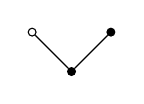
\begin{tikzpicture}[grow = up, level distance = 0.5cm, sibling distance = 1cm,every node/.style = {shape = circle, draw, inner sep = 1pt}]
            \node[fill = black] {}
                child{ node[fill = black]{} }
                child{ node[fill = white]{} };
         \end{tikzpicture}&\(\{fy\}\)&3&1\\
         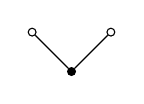
\begin{tikzpicture}[grow = up, level distance = 0.5cm, sibling distance = 1cm,every node/.style = {shape = circle, draw, inner sep = 1pt}]
            \node[fill = black] {}
                child{ node[fill = white]{} }
                child{ node[fill = white]{} };
         \end{tikzpicture}&\(\{y^2\}\)&3&2\\
         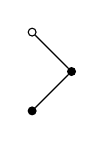
\begin{tikzpicture}[grow = up, level distance = 0.5cm, sibling distance = 1cm,every node/.style = {shape = circle, draw, inner sep = 1pt}]
            \node[fill = black] {}
                child{ node[fill = black]{} 
                    child[missing]{ node{} }
                    child{ node[fill = white]{} }}
                child[missing]{ node{} };
         \end{tikzpicture}&\(\{_2y\}_2\)&3&1\\
         \hline
    \end{tabular}
    \caption{Alle spookbomen \(t\) met \(\rho(t)\le3\).}
    \label{tab:ghosttrees}
\end{table}
De voorwaarde uit lemma \ref{lem:orderv1} om een methode van orde \(q\) te hebben is nu niet langer voldoende, er dient nu ook te gelden dat \(\psi(t)=0\) voor alle spookbomen \(t\) waarvoor \(\rho'(t)\le q\). Ook hier moet rekening gehouden worden met het feit dat de coëfficiënten in de spooktermen zelf in functie van \(h\) zijn en er dus herschikkingen nodig zijn. Uiteindelijk wordt het volgende resultaat bekomen:
\begin{lem} \label{lem:order}
Een gemodificeerde EFRK-methode is van orde \(q\) als en slechts als:
\begin{itemize}
    \item \(\psi(t)=\gamma(t)^{-1}+\mathcal{O}(h^{q+1-\rho(t)})\) voor alle bomen \(t\) tot en met orde \(q\).
    \item \(\psi(t)=\mathcal{O}(h^{q+1-\rho'(t)})\) voor alle spookbomen \(t\) waarvoor \(\rho'(t)\le q\).
\end{itemize}
\end{lem}
De sommatie over de spookbomen kan hier inzichtelijker gemaakt worden. Zoals eerder vermeld is voor de \(\delta_i\) de reeksontwikkeling in \(h\) minstens van orde \(\mathcal{O}(h^2)\). Elk voorkomen van een \(\delta_i\) in de uitdrukking \(\psi(t)\), of analoog het aantal voorkomens \(\rho_g(t)\) van de spookboom \(\tau_g\) als deelboom in een boom \(t\) (uit de definitie van \(\psi\)), verhoogt bijgevolg de orde van \(h\) in de term bij \(t\) met minstens twee. De totale orde van \(h\) wordt dan minstens \(\rho'(t)+2\rho_g(t)=\rho(t)+\rho_g(t)\) voor een zekere boom \(t\). De voorwaarde \(\psi(t)=\mathcal{O}(h^{q+1-\rho'(t)})\) moet dus enkel gecontroleerd worden voor bomen \(t\) met \(\rho(t)+\rho_g(t)\le q\).
\begin{vbn}
    Neem de spookboom \(t=[\tau_g]\). De bijbehorende spookterm wordt gegeven door:
    \[-\frac{h^{\rho'(t)}}{\sigma(t)}\psi(t)F(t)=-h\sum_{j=1}^sb_j\delta_j\{y\}.\]
    In eerste instantie lijkt het dus alsof deze term ook een bijdrage kan leveren aan de eerste-ordeterm van de reeksontwikkeling van de fout. De som bevat echter eenmaal \(\delta_j\), omdat \(\tau_g\) één keer voorkomt als deelboom en in de definitie van \(\psi\) elke \(\tau_g\) wordt omgezet in \(\delta_j\). Omdat \(\delta_j=\mathcal{O}(h^2)\), zal er uiteindelijk minstens \(h^3\) voorop staan, dus voor methodes van orde twee is \(\psi(t)=\mathcal{O}(h^{q+1-\rho'(t)})\) automatisch voldaan, ook al is \(\rho'(t)=1<q=2\).
\end{vbn}

\subsubsection{Herschikking}
Als een methode dan effectief van orde \(q\) is, dan zal de leidende term van de fout (ook lte genoemd, naar \textit{leading term error}) van de volgende vorm zijn:
\[lte=h^{q+1}\sum_{t\in\mathcal{T}\cup\mathcal{G}}c_tF(t).\]
De elementaire differentialen \(F(t)\) kunnen nu per orde verder gegroepeerd worden tot gewone afgeleiden van \(y\). In het klassieke geval kunnen voor de leidende term in de afknottingsfout de elementaire differentialen herschreven worden in termen van totale afgeleiden van aflopende ordes \(q+1\) tot en met \(r+1\) (zie \cite{stageorder}), waarbij \(r\) de traporde ven de methode is.
\begin{defn} \label{def:stageorder}
    De traporde van een \(s\)-traps RK-methode is de hoogst mogelijke \(r\) waarvoor geldt dat
    \[\sum^s_{j=1}a_{ij}c_j^{k-1}=\frac{c_i^k}{k},\qquad i=1,\dots,s,\qquad k=1,\dots,r.\]
\end{defn}
Hiermee kan gewerkt worden naar een meer inzichtelijke vorm van de leidende foutterm:
\[lte=h^{q+1}\sum^{q+1}_{i=r+1}c_i\times\text{`afgeleiden van \(f\)'}\times y^{(j)}.\]
De `afgeleiden van \(f\)' zijn dan jacobianen en andere Fréchetafgeleiden (zie \cite{gnm} voor een definitie van dit begrip).
\begin{vbn}
    Beschouw de trapeziumregel, een tweetrapsmethode gegeven door het volgende tableau:
    \[
    \renewcommand\arraystretch{1.2}
    \begin{array}
    {c|c|cc}
    0 & 1 & 0 & 0 \\
    1 & 1 & \frac{1}{2} & \frac{1}{2} \\
    \hline
    && \frac{1}{2} & \frac{1}{2}
    \end{array}
    \]
    Dit is methode van orde 2 en traporde 2 en de lte kan dus herschreven worden als een totale afgeleide van orde 3:
    \begin{align*}
        lte&=\frac{h^3}{3!}\sum_{\rho(t)=3}\alpha(t)[1-\gamma(t)\psi(t)]F(t) \\
        &=\frac{h^3}{3!}\left([1-3\psi([\tau^2])]\{f^2\}+[1-6\psi([_2\tau]_2)]\{_2f\}_2\right) \\
        &=\frac{h^3}{3!}\left([1-3\sum_ib_ic^2_i]\{f^2\}+[1-6\sum_{i,j}b_ia_{ij}c_j]\{_2f\}_2\right) \\
        &=\frac{h^3}{3!}\left(-\frac{1}{2}\{f^2\}-\frac{1}{2}\{_2f\}_2\right) \\
        &=-\frac{h^3}{12}(\{f^2\}+\{_2f\}_2) \\
        &=-\frac{h^3}{12}y^{(3)}.
    \end{align*}
\end{vbn}
Voor het exponentieel gefitte geval is het herschrijven in gewone afgeleiden niet altijd meer mogelijk. De definitie van de traporde houdt geen rekening met het feit dat de coëfficiënten ook functies van \(h\) zijn, dus de gelijkheid in definitie \ref{def:stageorder} zal maar gelden tot op een bepaalde orde van \(h\). Bovendien leveren bomen van lagere orde vaak ook nog een bijdrage aan de leidende foutterm. Het lukt echter vaak toch om een meer inzichtelijke vorm te verkrijgen.
\begin{vbn}
    De exponentieel gefitte versie van de trapeziumregel op \(S_{\textrm{ext}}=\{1,\exp(\mu_1x)\}\) wordt gegeven door het tableau
    \[
    \renewcommand\arraystretch{1.2}
    \begin{array}
    {c|c|cc}
    0 & 1 & 0 & 0 \\
    1 & 1 & b & b \\
    \hline
    && b & b
    \end{array}
    \]
    met \(b=\frac{\sinh\left(\frac{z_1}{2}\right)}{z_1\cosh\left(\frac{z_1}{2}\right)}\). De methode blijft van orde twee, maar de leidende foutterm wordt nu aangevuld met een bijdrage van de boom van orde één.
    \begin{align*}
        lte&=-\frac{h^3}{12}y^{(3)}+\frac{h}{1!}\sum_{\rho(t)=3}\alpha(t)[1-\gamma(t)\psi(t)]F(t) \\
        &=-\frac{h^3}{12}y^{(3)}+h\alpha(\tau)[1-\gamma(\tau)\psi(\tau)]F(\tau) \\
        &=-\frac{h^3}{12}y^{(3)}+h[1-\sum^s_{i=1}b_i]f \\
        &=-\frac{h^3}{12}y^{(3)}+h[1-(1-\frac{1}{12}z_1^2+\mathcal{O}(h^4))]f \\
        &=-\frac{h^3}{12}y^{(3)}+\frac{h}{12}z_1^2f \\
        &=\frac{h^3}{12}(\mu_1^2y^{(1)}-y^{(3)})
    \end{align*}
    De lte is nu ook afhankelijk van de eerste orde afgeleide van \(y\), maar er kan wel duidelijk worden afgelezen dat de keuze \(\mu_1^2=\frac{y^{(3)}}{y^{(1)}}\) de leidende foutterm (en ook de andere termen) nul maakt, of dus dat de methode inderdaad exact is voor \(\exp(\mu_1x)\).
\end{vbn}

\subsection{Stabiliteit}
Nog een wenselijke eigenschap voor numerieke methoden is dat hun oplossingen hetzelfde gedrag vertonen op oneindig als de exacte oplossing: convergeert de numerieke oplossing naar nul als de exacte oplossing dat doet? Om op deze vraag te antwoorden wordt gebruik gemaakt van een testvergelijking:
\begin{equation} \label{eq:testeq}
    y'(x)=\omega y(x),\qquad\omega\in\mathbb{C}^-.
\end{equation}
De exacte oplossing van deze testvergelijking is \(y=\exp(\omega x)+c\) en convergeert inderdaad slechts naar 0 voor \(x\to\infty\) op voorwaarde dat \(\omega\) in het complexe linkerhalfvlak ligt. Om te kijken wat er in het numerieke geval gebeurt, wordt gekeken naar het gedrag van de zogenaamde stabiliteitsveelterm \(R(z)\). Hier is \(z=\omega h\) een complex getal in functie van de frequentie \(\omega\) van de testvergelijking en de stapgrootte \(h\) van de methode. Voor een gemodificeerde RK-methode wordt de stabiliteitsveelterm gegeven door de volgende formule:
\begin{equation} \label{eq:stability}
    R(z)=1+zb^\top(I-zA)^{-1}\Gamma.
\end{equation}
De coëfficiënten, bevat in \(A\), \(b\) en \(\Gamma\), zijn bij EFRK-methodes afhankelijk van de frequenties waarop gefit wordt en die afhankelijkheid wordt dan ook doorgetrokken naar \(R(z)\) (impliciet staat er dus \(R(z,\mu_1,\dots,\mu_l)\)). Voor deze veelterm geldt nu dat
\begin{equation*}
    y_{n+1}=R(z)y_n=R(z)^{n+1}y_0.
\end{equation*}
Hiermee is het duidelijk dat de convergentie op oneindig van de numerieke oplossing pas gewaarborgd is indien \(|R(z)|<1\). Er moet dus gezocht worden naar het gebied van absolute stabiliteit:
\begin{equation} \label{eq:absstab}
    \mathcal{R}_A=\{z\;|\;|R(z)|<1\}.
\end{equation}
Is \(\mathbb{C}^-\) bevat in \(\mathcal{R}_A\), dan is het gedrag op oneindig dus overeenkomstig en spreekt men van een absoluut stabiele of A-stabiele methode. Indien de eigenschap \(\mathbb{C}^-=\mathcal{R}_A\) geldt, dan wordt de methode exact-A-stabiel genoemd.

\newpage
\section{Tweetrapsmethode} \label{sec:rks2}
\subsection{De methode}
De standaard tweetraps gemodificeerde RK-methode ziet er als volgt uit:
\[
\renewcommand\arraystretch{1.2}
\begin{array}
{c|c|cc}
c_1 & \gamma_1 & a_{11} & a_{12} \\
c_2 & \gamma_2 & a_{21} & a_{22} \\
\hline
&& b_1 & b_2 
\end{array}
\]
De symmetrievoorwaarden worden hier
\[\systeme*{c_1=1-c_2,\gamma_1=\gamma_2=\gamma,b_1=b_2=b,a_{11}=\gamma b-a_{22},a_{12}=\gamma b-a_{21}}\]
en hiervan gebruik makend vertaalt de symplecticiteit zich in het volgende stelsel:
\[\systeme*{\frac{b}{\gamma}a_{11}=b^2-\frac{b}{\gamma}a_{11},\frac{b}{\gamma}a_{21}=b^2-\frac{b}{\gamma}a_{12},\frac{b}{\gamma}a_{22}=b^2-\frac{b}{\gamma}a_{22}}\]
Deze twee stelsels worden vervolgens samengenomen en herschreven met behulp van twee andere parameters \(\lambda\) en \(\theta\). Deze weerspiegelen beter de symmetrie en maken de resultaten later duidelijker. De volgende coëfficiënten worden dan verkregen:
\[\systeme*{c_1=\frac{1}{2}-\theta,c_2=\frac{1}{2}+\theta,a_{11}=\frac{\gamma b}{2},a_{12}=\frac{\gamma b}{2}+\lambda,a_{21}=\frac{\gamma b}{2}-\lambda,a_{22}=\frac{\gamma b}{2}}\]
of in tableau-vorm:
\begin{equation} \label{eq:rks2}
\renewcommand\arraystretch{1.2}
\begin{array}
{c|c|cc}
\frac{1}{2}-\theta & \gamma & \frac{\gamma b}{2} & \frac{\gamma b}{2}+\lambda \\
\frac{1}{2}+\theta & \gamma & \frac{\gamma b}{2}-\lambda & \frac{\gamma b}{2} \\
\hline
&& b & b 
\end{array}
\end{equation}
Elke RK-methode integreert een constante functie exact (zie ook opmerking \ref{opm:consistent}). Verder wordt op de interne trappen en de externe trap de functie \(\exp(\pm\mu_1x)\), met \(\mu_1=\omega_1\vee i\omega_1,\omega_1\in\mathbb{R}^+\), opgelegd, of met andere woorden:
\[S_{\textrm{int}}=\{\exp(\pm\mu_1x)\},\qquad S_{\textrm{ext}}=\{1,\exp(\pm\mu_1x)\}.\]
Met behulp van de functionalen \(\mathcal{L}_i\) en \(\mathcal{L}\) uit (\ref{eq:functionals}) toegepast op de functie \(\exp(\pm\mu_1x)\) worden de coëfficiënten:
\begin{equation} \label{eq:rks2coeff}
    b=\frac{\sinh(\frac{z_1}{2})}{\cosh(z_1\theta)z_1},\qquad\gamma=\frac{\cosh(2z_1\theta)}{\cosh(\frac{z_1}{2})\cosh(z_1\theta)},\qquad\lambda=-\frac{\sinh(z_1\theta)}{\cosh(z_1\theta)z_1}.
\end{equation}
Hierbij is \(z_1=\mu_1h\). Er is dus nog één vrijheidsgraad, \(\theta\), die kan vastgelegd worden door de functie \(\exp(\pm\mu_2x)\), met opnieuw \(\mu_2=\omega_2\vee i\omega_2,\omega_2\in\mathbb{R}^+\), op te leggen voor de externe trap:
\[S_{\textrm{int}}=\{\exp(\pm\mu_1x)\},\qquad S_{\textrm{ext}}=\{1,\exp(\pm\mu_1x),\exp(\pm\mu_2x)\}.\]
Dit levert dezelfde voorwaarde op voor \(b\) in \(z_2=\mu_2h\), waardoor \(\theta\) kan bepaald worden uit:
\[\frac{\sinh(\frac{z_1}{2})}{\cosh(z_1\theta)z_1}=\frac{\sinh(\frac{z_2}{2})}{\cosh(z_2\theta)z_2}.\]
Met behulp van de eta-functies van Ixaru kan dit ook als volgt geschreven worden:
\begin{equation} \label{eq:thetaeq}
    \frac{\eta_0(\frac{Z_1}{4})}{\eta_{-1}(Z_1\theta^2)}=\frac{\eta_0(\frac{Z_2}{4})}{\eta_{-1}(Z_2\theta^2)}.
\end{equation}
Definiëren we nu
\[F(Z,\theta)=\frac{\eta_0(\frac{Z}{4})}{\eta_{-1}(Z\theta^2)},\]
dan kan de voorwaarde eenvoudig worden voorgesteld als \(F(Z_1,\theta)-F(Z_2,\theta)=0\). Er bestaat jammer genoeg geen oplossing voor deze vergelijking in expliciete vorm, dus de bepaling van \(\theta\) zal via numerieke benaderingen moeten gebeuren. Een mogelijke manier hierbij is om te werken met de verhouding van beide frequenties:
\[\alpha=\frac{Z_2}{Z_1}=\frac{\mu_2^2}{\mu_1^2}.\]
Bij positieve waarden van \(\alpha\) zijn de frequenties allebei reëel of complex, bij negatieve waarden komt zowel een reële als een complexe frequentie voor. Voor verschillende waarden van \(\alpha\) kan de vergelijking \(G(Z,\theta)=F(Z,\theta)-F(\alpha Z,\theta)=0\) numeriek worden opgelost. Het resultaat hiervan voor \(Z_i\in[-5,5]\) wordt geplot in figuur \ref{fig:thetagraph}. Merk op dat de vergelijking voor \(\theta\) symmetrisch is in beide frequenties en dit dus ook weerspiegeld wordt in deze grafiek.
\begin{nta}
In de numerieke resultaten zal voor deze methode de naam RKs2 gebruikt worden.
\end{nta}
\begin{figure}[H]
    \centering
    \includegraphics[width=0.7\textwidth]{thetagraph.jpg}
    \caption{\(\theta\) in functie van \(Z_1\) en \(Z_2\).}
    \label{fig:thetagraph}
\end{figure}
Vaak wordt ook de vraag gesteld wat er gebeurt wanneer de integratiepunten \(c_i\) op voorhand vast worden genomen, meestal op de gaussische knooppunten, wat correspondeert met \(\theta=\frac{\sqrt{3}}{6}\) in het geval van de tweetrapsmethode. Gezien hierdoor een vrijheidsgraad verloren is, kan er niet meer gefit worden op een extra frequentie \(\mu_2\), maar impliciet legt de keuze van een constante \(\theta\) toch een tweede \(z_2\) vast die door de externe trap exact wordt geïntegreerd: de snijlijn van het impliciete oppervlak uit figuur \ref{fig:thetagraph} en het vlak \(\theta=\frac{\sqrt{3}}{6}\). Voor kleine waarden van \(z_1\) leunt \(z_2\) nauw aan tegen \(iz_1\), waardoor het lijkt alsof de externe trappen zowel een exponentiële als een goniometrische component exact integreren. Dit alles wordt geïllustreerd in figuur \ref{fig:consthetarks2}: de blauwe kromme is de vermelde doorsnede en ligt inderdaad dicht bij het geval \(Z_2=-Z_1\), equivalent met \(z_2=\pm iz_1\). Een uitgebreide behandeling van deze versie van de methode kan teruggevonden worden in \cite{4thordersympl}.
\begin{figure}[H]
    \centering
    \includegraphics[width=0.7\textwidth]{cons_theta_RKs2.jpg}
    \caption{De ligging van \(\theta=\frac{\sqrt{3}}{6}\) en verwante waarden, met \(\delta=0.001\).}
    \label{fig:consthetarks2}
\end{figure}

\subsection{Coëfficiënten} \label{subsec:coeff}
Een eerste observatie omtrent de coëfficiënten volgt al uit figuur \ref{fig:thetagraph}: \(\theta\) lijkt als functie van \(z_1\) en \(z_2\) niet heel variabel. Omdat de \(z_i\) vaak schattingen zijn met een zekere foutmarge, is dit een zeer handige eigenschap. Naarmate de verhouding \(\alpha\) in absolute waarde toeneemt, neemt variatie wel toe. De andere coëfficiënten, geplot in hetzelfde interval als \(\theta\) in figuur \ref{fig:coefgraphs}, zijn iets meer variabel, voornamelijk \(\gamma\) voor sterk negatieve \(Z_1\), maar verder vertonen ze geen problematisch gedrag. 

Er ontstaat echter een ander probleem bij negatieve \(Z_i\): in principe is \(\theta\) bepaald over geheel \(\mathbb{R}^2\), maar in het geval dat een \(Z_i\) negatief wordt en de corresponderende \(z_i\) dus imaginair, komen er in de bepaling van de parameters cosinussen met nulpunten. Dit wordt geïllustreerd in figuur \ref{fig:contourplot}, waar de nulpunten worden geplot van vergelijking (\ref{eq:thetaeq}) voor \(z_2=2z_1\) met behulp van een contourplot. Slechts drie van de vijf krommen op de figuur stellen wel degelijk nulpunten voor, de twee andere lijnen zijn fouten ten gevolge van de polen van de vergelijking (ontstaan door de nulpunten van de cosinussen in de noemer). Figuur \ref{fig:contourplotex}, die een doorsnede weergeeft voor het geval \(Z_1=-5\), verduidelijkt dit: de rode kromme heeft slechts twee nulpunten in het interval \([0,1]\) en twee verticale asymptoten. Wanneer nu een dergelijke poollijn uit het contourplot snijdt met een werkelijke contour, dan ontstaan er soms sprongen naar een andere contour bij de numerieke bepaling van \(\theta\). In theorie kunnen verschillende van deze discontinuïteiten relatief eenvoudig weggewerkt worden, met behulp van l'Hopital, maar een aparte numerieke behandeling bij al deze gevallen is allerminst wenselijk. Bovendien treden dergelijke discontinuïteiten ook op bij de coëfficiënten en naarmate de verhouding \(|\alpha|\) groter wordt, treden ze zelfs eerder op. Bijgevolg is de methode praktisch niet meer bruikbaar voor grote imaginaire \(z_i\). Dit alles maakt dat het toepassen van de methode best beperkt blijft tot relatief kleine frequenties.

\begin{figure}[H]
\begin{subfigure}{0.49\textwidth}
\includegraphics[width=0.9\linewidth]{b_s2.jpg} 
\end{subfigure}
\begin{subfigure}{0.49\textwidth}
\includegraphics[width=0.9\linewidth]{gamma_s2.jpg}
\end{subfigure}
\begin{center}
\begin{subfigure}{0.5\textwidth}
\includegraphics[width=0.9\linewidth]{lambda_s2.jpg} 
\end{subfigure}
\end{center}
\caption{Het verloop van de verschillende coëfficiënten in functie van de gefitte parameters.}
\label{fig:coefgraphs}
\end{figure}

\begin{figure}[H]
    \begin{subfigure}{0.49\textwidth}
    \includegraphics[width=0.9\linewidth]{contour_theta_RKs2.jpg} 
    \subcaption{Contourplot uit vergelijking (\ref{eq:thetaeq})}
    \label{fig:contourplot}
    \end{subfigure}
    \begin{subfigure}{0.49\textwidth}
    \includegraphics[width=0.9\linewidth]{contour_theta_RKs2_ex.jpg}
    \subcaption{Doorsnede voor \(Z_1=-5\)}
    \label{fig:contourplotex}
    \end{subfigure}
    \caption{Illustratie van de nulpunten en polen bij de bepaling van \(\theta\).}
\end{figure}

Zoals bij alle exponentieel gefitte methoden kunnen kleine waarden van \(z_i\) zorgen voor fouten bij het berekenen van de coëfficiënten. De frequenties komen immers in teller en noemer van alle uitdrukkingen voor, waardoor kleine getallen met afrondingsfouten door elkaar gedeeld worden. Daarom is het beter om vanaf een zekere grenswaarde voor \(|z_i|\), vaak 0.1 gekozen, de reeksontwikkelingen van de coëfficiënten te gebruiken. Voor \(\theta\) geeft dit het volgende resultaat:
\begin{equation} \label{eq:thetas2series}
    \begin{split}
        \theta=\frac{\sqrt{3}}{6}&+\frac{\sqrt{3}}{2160}(z_1^2+z_2^2)-\frac{\sqrt{3}}{10886400}(27z_1^4-106z_1^2z_2^2+27z_2^4) \\
        &+\frac{\sqrt{3}}{435456000}(3z_1^4-34z_1^2z_2^2+3z_2^4)(z_1^2+z_2^2)+\dots
    \end{split}
\end{equation}
Met behulp hiervan kunnen ook de andere drie parameters benaderd worden met een reeksontwikkeling:
\begin{equation} \label{eq:bs2series}
\begin{split}
    b=\frac{1}{2}+\frac{z_1^2(z_1^2-252)z_2^2}{2177280}+&\frac{(-244500z_1^6 + 21168000z_1^4+435456000z_1^2)z_2^4}{948109639680000} \\ &+\frac{(-3943z_1^6-91320z_1^4)z_2^6}{948109639680000}+\dots
\end{split}
\end{equation}
\begin{equation} \label{eq:ls2series}
\begin{split}
    \lambda=-\frac{\sqrt{3}}{6}+\frac{\sqrt{3}z_1^2}{240}-\frac{137\sqrt{3}z_1^4}{1209600}+&\frac{143\sqrt{3}z_1^6}{48384000}+\left(-\frac{\sqrt{3}}{2160} +\frac{157\sqrt{3}z_1^2}{5443200}-\frac{1367\sqrt{3}z_1^4}{1306368000}\right)z_2^2 \\ &+\left(\frac{\sqrt{3}}{403200} - \frac{37\sqrt{3}z_1^2}{1306368000}\right)z_2^4- \frac{\sqrt{3}z_2^6}{145152000}+\dots
\end{split}
\end{equation}
\begin{equation} \label{eq:gs2series}
    \gamma=1-\frac{z_1^4}{360}+\frac{11z_1^6}{30240}+\left(\frac{z_1^2}{1440}-\frac{29z_1^4}{362880}\right)z_2^2-\frac{z_1^2z_2^4}{362880}+\dots
\end{equation}
Wegens het multiparametrisch karakter van de methode is het nu echter mogelijk dat slechts één van beide frequenties onder de grenswaarde ligt. Hier kunnen reeksontwikkelingen in enkel de probleemfrequentie gebruikt worden. Indien in het bijzonder enkel \(z_2\) zeer klein is, dient enkel een benadering gebruikt te worden voor \(\theta\). De overige coëfficiënten, gedefinieerd in (\ref{eq:rks2coeff}), zijn immers enkel onrechtstreeks afhankelijk van \(z_2\) via \(\theta\).

\subsection{Foutterm}
De orde van methode (\ref{eq:rks2}) volgt uit lemma \ref{lem:order}: de laagste-ordetermen in \(h\) treden op vanaf orde vijf, zowel bij de sommatie over de gewone bomen als over de spookbomen. Hieronder worden alle bomen tot en met orde vijf en de spookbomen overlopen en wordt de bijdrage aan de foutterm berekend.

\subsubsection{Bomen van orde één}
Er is slechts één boom van orde één, namelijk \(\tau\). De factor \(\frac{h}{1!}\) draagt al één bij om tot een vijfde-ordeterm te komen, bijgevolg dient op zoek gegaan te worden naar de vierde-ordeterm in \(h\) van de reeksontwikkeling van \(\psi(\tau)\). Dit geeft als resultaat
\[\frac{h^5}{4320}\mu_1^2\mu_2^2f,\]
of in termen van gewone afgeleiden
\[\frac{h^5}{4320}\mu_1^2\mu_2^2y^{(1)}.\]
\subsubsection{Bomen van orde twee}
De orde van \(h\) voorop in de sommatie is nu twee, waardoor een mogelijke bijdrage aan de vijfde-ordeterm nu moet komen van de derde-ordeterm van de reeksontwikkeling van \(\psi(t)\), met \(t\) een boom van orde twee. Deze reeksontwikkeling is echter zoals eerder afgeleid even, dus deze bomen hebben geen effect op de lte.
\subsubsection{Bomen van orde drie}
Uit een analoge redenering als bij de bomen van orde een volgt dat op zoek dient gegaan te worden naar de tweede-ordetermen van de reeksontwikkelingen van \(\psi(t)\), \(\rho(t)=3\). De bomen en hun corresponderende term zijn de volgende: 
\begin{itemize}
    \item \([\tau^2]\Rightarrow\frac{h^5}{4320}\left(9\mu_1^2-\mu_2^2\right)\{f^2\}\)
    \item \([_2\tau]_2\Rightarrow\frac{h^5}{2160}\left(\mu_2^2-9\mu_1^2\right)\{_2f\}_2\)
\end{itemize}
Groeperen in termen van gewone afgeleiden geeft:
\[\frac{h^5}{4320}(9\mu_1^2-\mu_2^2)(y^{(3)}-3Jy^{(2)}).\]
\subsubsection{Bomen van orde vier}
Net als bij orde twee is de relevante term, nu die van eerste orde, gelijk aan nul.
\subsubsection{Bomen van orde vijf}
Nu de factor voorop al \(h^5\) is, dienen enkel nog de constante termen in de ontwikkelingen van \(\psi(t)\) berekend te worden, met als resultaat:
\begin{itemize}
    \item \([\tau^4]\Rightarrow\frac{h^5}{4320}\{f^4\}\)
    \item \([[\tau]^2]\Rightarrow\frac{h^5}{1440}\{\{f\}^2\}\)
    \item \([\tau[\tau^2]]\Rightarrow-\frac{h^5}{720}\{f\{f^2\}\}\)
    \item \([\tau[_2\tau]_2]\Rightarrow-\frac{h^5}{720}\{f\{_2f\}_2\}\)
    \item \([\tau^2[\tau]]\Rightarrow\frac{h^5}{720}\{f^2\{f\}\}\)
    \item \([_2\tau^3]_2\Rightarrow-\frac{h^5}{1080}\{_2f^2\}\)
    \item \([_2\tau[\tau]]_2\Rightarrow-\frac{h^5}{360}\{_2f\{f\}\}_2\)
    \item \([_3\tau^2]_3\Rightarrow\frac{h^5}{720}\{_3f^2\}_3\)
    \item \([_4\tau]_4\Rightarrow\frac{h^5}{720}\{_4f\}_4\)
\end{itemize}
Sommeren en herschrijven geeft
\[\frac{h^5}{4320}(10J^2y^{(3)}-5Jy^{(4)}+y^{(5)}-10\mathbf{f}(y^{(1)},y^{(3)})),\]
waarbij \(\mathbf{f}\) de tweede Fréchetafgeleide van \(f\) voorstelt.
\subsubsection{Spookbomen}
De relevante spookbomen \(t\) zijn diegene waarvoor \(\rho(t)+\rho_g(t)\le 4\), of dus \([\tau_g]\), \([_2\tau_g]_2\) en \([\tau\tau_g]\). Voor de twee bomen van orde drie, \([_2\tau_g]_2\) en \([\tau\tau_g]\), geldt echter dat \(\rho'(t)=2\) en dus dat de orde van \(h\) voorop in de term twee is. Net zoals bij de gewone bomen van even orde betekent dit dat de relevante ordetermen nul zijn en dus blijft enkel \([\tau_g]\) over. De spookterm die daaruit volgt is
\[\frac{h^5}{1440}\left(4\mu_1^4-\mu_1^2\mu_2^2\right)f=\frac{h^5}{1440}\left(4\mu_1^4-\mu_1^2\mu_2^2\right)y^{(1)}.\]
\subsubsection{Interpretatie}
Indien we al deze termen bij elkaar nemen, dan wordt de volgende uitdrukking voor de foutterm verkregen:
\begin{equation}\label{eq:error}
\begin{split}
    y(x_n)-y_n=&\frac{h^5}{4320}\Big((12\mu_1^4-2\mu_1^2\mu_2^2)y^{(1)}+(9\mu_1^2-\mu_2^2)(y^{(3)}-3Jy^{(2)}) \\
    & +10J^2y^{(3)}-5Jy^{(4)}+y^{(5)}-10\mathbf{f}(y^{(1)},y^{(3)})\Big)+\mathcal{O}(h^6),
\end{split}
\end{equation}
Met behulp hiervan zou nu op zoek gegaan kunnen worden naar de optimale parameters \(\mu_i\), gegeven een functie \(y\): zoek goeie benaderingen voor \(y^{(2)},y^{(3)},y^{(4)}\) en \(y^{(5)}\) om vervolgens de leidende foutterm te minimaliseren over alle mogelijke parameterwaarden. In de realiteit zijn dergelijke benaderingen moeilijk te vinden, omdat de uitdrukking voor \(y\) niet gekend is. Toch kunnen in (\ref{eq:error}) al twee dingen herkend worden:
\begin{itemize}
    \item Indien \(\mu_1=\mu_2=0\) worden gekozen, komt de foutterm overeen met die van de klassieke gaussische tweetrapsmethode, zoals gevonden in \cite{EFRKfixedvar}.
    \item Neem de vergelijking \(y'=\omega y\), met als oplossing \(y=\exp(\omega x)\), dan vereenvoudigt (\ref{eq:error}) tot
    \[y(x_n)-y_n=\frac{h^5}{2160}(6\mu^4_1-\mu_1^2\mu_2^2-9\mu_1^2\omega^2+\mu_2^2\omega^2+3\omega^4)y^{(1)}+\mathcal{O}(h^6).\]
    De middelste factor van de lte factoriseert verder tot \((\mu_1^2-\omega^2)(\mu_1^2-\frac{\mu_2^2+3\omega^2}{6})\), dus \(\mu_1=\pm\omega\) maakt de leidende foutterm nul. Ook de andere fouttermen zullen nul worden, consistent met het feit dat de interne en externe trappen de frequentie \(\mu_1\) exact integreren.
\end{itemize}
Bij de numerieke voorbeelden in hoofdstuk \ref{sec:numericex} worden verdere pogingen ondernomen om de foutterm te interpreteren.

\subsection{Stabiliteit}
De stabiliteitsfunctie wordt met behulp van (\ref{eq:stability}):
\begin{equation}
    R(z)=\frac{1+\gamma b z+\lambda^2z^2}{1-\gamma b z+\lambda^2z^2}.
\end{equation}
De grens van het gebied van absolute stabiliteit \(\mathcal{R}_A\) wordt als volgt bepaald (met \(z=x+iy\)):
\begin{equation*}
    \begin{split}
        |R(z)|&=1\\
        \Leftrightarrow|1+\gamma b z+\lambda^2z^2|&=|1-\gamma b z+\lambda^2z^2| \\
        \Leftrightarrow|1+\gamma b z+\lambda^2z^2|^2&=|1-\gamma b z+\lambda^2z^2|^2 \\
        \Leftrightarrow|(1+\gamma bx+\lambda^2(x^2-y^2))+iy(\gamma b+2x\lambda^2)|^2&=|(1-\gamma bx+\lambda^2(x^2-y^2))+iy(2x\lambda^2-\gamma b)|^2 \\
        \Leftrightarrow(1+\gamma bx+\lambda^2(x^2-y^2))^2+y^2(\gamma b+2x\lambda^2)^2&=(1-\gamma bx+\lambda^2(x^2-y^2))^2+y^2(2x\lambda^2-\gamma b)^2 \\
        \Leftrightarrow2\gamma bx+2\gamma bx\lambda^2(x^2-y^2)+4\gamma bx\lambda^2y^2&=-2\gamma bx-2\gamma bx\lambda^2(x^2-y^2)-4\gamma bx\lambda^2y^2 \\
        \Leftrightarrow x+x\lambda^2(x^2-y^2)+2x\lambda^2y^2&=0 \\
        \Leftrightarrow x(1+\lambda^2(x^2+y^2))&=0
    \end{split}
\end{equation*}
De tweede factor in de finale gelijkheid is strikt positief, waardoor de oplossing \(x=0\) wordt, of dus de imaginaire as. Bij deze berekening is enkel gesteund op het feit dat het product \(\gamma b\) niet nul is, wat wel het geval kan zijn voor imaginaire \(z_i\): er komt dan een sinus in de teller van \(b\) en een cosinus in de teller van \(\gamma\) en beide hebben nulpunten, gegeven door:
\[z_1=\frac{(2j+1)\pi i}{4\theta},\quad j\in\mathbb{Z}\quad\vee\quad z_1=2j\pi i, \quad j\in\mathbb{Z}^0.\]
In deze nulpunten vereenvoudigt de stabiliteitsfunctie tot \(R(z)=1\), onafhankelijk van \(z\), en het stabiliteitsgebied wordt \(\varnothing\). Dit resulteert dus zelfs niet meer in een methode die een veralgemening is van een klassieke eerste-orde-methode (waarvoor \(R(z)\) dus \(\exp(z)\) minstens tot op eerste orde benadert). De tweetrapsmethode wordt dus nutteloos bij dergelijke keuzes voor \(z_i\) en bovendien ontstaan er nog problematische gevallen. Om te kijken waar ten opzichte van de imaginaire as het stabiliteitsgebied nu precies ligt, kan gekeken worden naar \(|R(-1)|\), of dus:
\[\left|\frac{\gamma b-\lambda^2-1}{\gamma b+\lambda^2+1}\right|.\]
Deze waarde is kleiner dan één (en \(-1\) ligt dus in \(\mathcal{R}_A\)) als en slechts als \(\gamma b\) positief is. Hieruit volgt dus dat het stabiliteitsgebied \(\mathbb{C}^-\) is als en slechts als \(\gamma b\) positief is. In figuur \ref{fig:stabrks2gb} wordt dit product weergegeven voor \(z_1\in[0,20i]\), waarop duidelijk negatieve zones te zien zijn. Hierdoor wisselt bij elke overgang van positief naar negatief het stabiliteitsgebied van \(\mathbb{C}^-\) naar \(\mathbb{C}^+\) en omgekeerd, zoals geïllustreerd in figuur \ref{fig:stabrks2imag}. 
\begin{figure}[H]
    \centering
    \includegraphics[width=0.5\textwidth]{stabrks2gb.jpg}
    \caption{Het verloop van \(\gamma b\) voor \(z_1\in[0,20i]\) en \(\theta=\frac{\sqrt{3}}{6}\).}
    \label{fig:stabrks2gb}
\end{figure}
\begin{figure}[H]
    \centering
    \begin{subfigure}{0.24\textwidth}
        \includegraphics[width=0.9\linewidth]{stabrks2_2i.jpg}
        \subcaption{\(z_1=2i\)}
    \end{subfigure}
    \begin{subfigure}{0.24\textwidth}
        \includegraphics[width=0.9\linewidth]{stabrks2_3i.jpg}
        \subcaption{\(z_1=3i\)}
    \end{subfigure}
    \begin{subfigure}{0.24\textwidth}
        \includegraphics[width=0.9\linewidth]{stabrks2_4i.jpg}
        \subcaption{\(z_1=4i\)}
    \end{subfigure}
    \begin{subfigure}{0.24\textwidth}
        \includegraphics[width=0.9\linewidth]{stabrks2_7i.jpg}
        \subcaption{\(z_1=7i\)}
    \end{subfigure}
    \caption{Stabiliteitsgebieden (turquoise) voor verschillende waarden van \(z_1\).}
    \label{fig:stabrks2imag}
\end{figure}
Voor reële frequenties wordt het gebied van absolute stabiliteit dus steeds gegeven door \(\mathbb{C}^-\) en is de methode onvoorwaardelijk exact-A-stabiel. Merk op dat hier de stabiliteitseigenschap van de klassieke gaussische methode, die eveneens exact-A-stabiel is, wordt overgeërfd. Voor imaginaire frequenties hangt de stabiliteit sterk af van de \(z_i\) en schommelt de methode tussen exacte A-stabiliteit, exacte A-instabiliteit en helemaal geen stabiliteit. Omdat deze schommelingen niet voorkomen bij kleine waarden van \(|z_i|\), is het dus ook om stabiliteitsredenen verstandig om het gebruik van de tweetrapsmethode te beperken tot relatief kleine frequenties.

\subsection{Speciale gevallen}
Voor enkele specifieke keuzes van \(z_2\) worden reeds gekende methodes verkregen. Wanneer bijvoorbeeld beide frequenties gelijk worden gekozen, resulterend in \(z_2=z_1\), dan wordt de voorwaarde ter bepaling van \(\theta\) gegeven door \(\frac{\partial F(Z,\theta)}{\partial Z}\bigr|_{Z=Z_1}=0\), wat vereenvoudigt tot:
\begin{equation} \label{eq:rks2z2=z1}
    \theta=\frac{\cosh(z_1\theta)}{z_1\sinh(z_1\theta)}\left(\frac{z_1\cosh(\frac{z_1}{2})}{2\sinh(\frac{z_1}{2})}-1\right).
\end{equation}
Deze specifieke versie werd al eerder onderzocht door Van den Berghe et al. in \cite{EFRKrevisited}. Een tweede optie die hierin voorkomt is die waarbij de tweede frequentie wordt ingeruild voor een hogere polynomiale orde, corresponderend met \(z_2=0\). Aangezien \(F(0,\theta)=1\), wordt de vergelijking ter bepaling van \(\theta\) nu \(F(Z_1,\theta)=1\), waarvoor een expliciete oplossing bestaat:
\begin{equation} \label{eq:rks2z2=0}
    \theta=\frac{1}{z_1}\arccos\left(\frac{2\sinh(\frac{z_1}{2})}{z_1}\right).
\end{equation}

Het geval waarbij de tweede frequentie het dubbele is van de eerste, of dus \(z_2=2z_1\), is nog niet specifiek onderzocht, maar geeft ook een exacte oplossing voor \(\theta\):
\begin{equation} \label{eq:rks2z2=2z1}
    \theta=\frac{1}{z_1}\arccos\left(\frac{\cosh\left(\frac{z_1}{2}\right)+\sqrt{8+\cosh\left(\frac{z_1}{2}\right)^2}}{4}\right).
\end{equation}
Het verloop van \(\theta\) wordt voor elk van deze speciale gevallen weergegeven in figuur \ref{fig:rks2specials}, die nogmaals illustreert dat een grotere \(|\alpha|\) voor een variabelere \(\theta\) zorgt, en dus een nauwkeurigere schatting van de \(z_i\) vereist. Het spreekt voor zich dat alle resultaten die tot nu toe zijn bekomen eveneens gelden voor deze specifieke gevallen door hun respectievelijke keuzes van \(z_2\) in te voegen.
\begin{figure}[H]
    \centering
    \includegraphics[width=0.7\textwidth]{specials_RKs2.jpg}
    \caption{Het verloop van \(\theta\) voor enkele speciale gevallen van \(z_2\).}
    \label{fig:rks2specials}
\end{figure}

\newpage
\section{Drietrapsmethode} \label{sec:rks3}
\subsection{De methode}
Een drietraps gemodificeerde RK-methode is van de vorm:
\[
\renewcommand\arraystretch{1.2}
\begin{array}
{c|c|ccc}
c_1 & \gamma_1 & a_{11} & a_{12} & a_{13} \\
c_2 & \gamma_2 & a_{21} & a_{22} & a_{23} \\
c_3 & \gamma_3 & a_{31} & a_{32} & a_{33} \\
\hline
&& b_1 & b_2 & b_3
\end{array}
\]
Als hierop symmetrievoorwaarden worden opgelegd voldoen de coëfficiënten aan het volgende stelsel:
\[\systeme*{c_1=1-c_3,c_2=\frac{1}{2},\gamma_1=\gamma_3,b_1=b_3,a_{11}=\gamma_1 b_1-a_{33},a_{12}=\gamma_1 b_2-a_{32},a_{13}=\gamma_1 b_1-a_{31},a_{21}=\gamma_2 b_1-a_{23},a_{22}=\frac{\gamma_2 b_2}{2}}\]
en de bijkomende voorwaarden die uit symplecticiteit volgen zijn:
\begin{equation*}
    \begin{cases}
        a_{11}&=\frac{b_1\gamma_1}{2} \\
        \frac{b_2}{\gamma_2}a_{21}&=b_1b_2-\frac{b_1}{\gamma_1}a_{12} \\
        \frac{b_1}{\gamma_1}a_{32}&=b_1b_2-\frac{b_2}{\gamma_2}a_{23} \\
        a_{33}&=\frac{b_1\gamma_1}{2}
    \end{cases}
\end{equation*}
Indien we opnieuw enkele andere parameters, \(\theta\), \(\alpha_2\) en \(\alpha_3\), invoeren die de resultaten later duidelijker gaan maken en de voorwaarden verder vereenvoudigen, bekomen we de volgende methode in tableau-vorm:
\begin{equation} \label{eq:rks3}
\renewcommand\arraystretch{1.2}
\begin{array}
{c|c|ccc}
\frac{1}{2}-\theta & \gamma_1 & \frac{\gamma_1 b_1}{2} & \frac{\gamma_1 b_2}{2}-\alpha_2 & \frac{\gamma_1 b_1}{2}-\alpha_3 \\
\frac{1}{2} & \gamma_2 & \frac{\gamma_2 b_1}{2}+\frac{b_1\alpha_2\gamma_2}{\gamma_1b_2} & \frac{\gamma_2 b_2}{2} &  \frac{\gamma_2 b_1}{2}-\frac{b_1\alpha_2\gamma_2}{\gamma_1b_2} \\
\frac{1}{2}+\theta & \gamma_1 & \frac{\gamma_1 b_1}{2}+\alpha_3 & \frac{\gamma_1 b_2}{2}+\alpha_2 & \frac{\gamma_1 b_1}{2} \\
\hline
&& b_1 & b_2 & b_1 
\end{array}
\end{equation}
Om tot concrete waarden te komen, kan er opnieuw gestart worden met het opleggen van de functie \(\exp(\pm\mu_1x)\), \(\mu_1\in\mathbb{C}\), voor alle trappen (bovenop de constante functie die opnieuw standaard is), of dus:
\[S_{\textrm{int}}=\{\exp(\pm\mu_1x)\},\qquad S_{\textrm{ext}}=\{1,\exp(\pm\mu_1x)\}.\]
Het oplossen van deze voorwaarden levert nu echter nog geen eenvoudige uitdrukkingen op in één resterende parameter \(\theta\), zoals in het tweetrapsgeval, en is ook nog afhankelijk van de parameters \(\gamma_1\) en \(\gamma_2\). Om die laatste twee weg te werken zijn dus bijkomende voorwaarden nodig, en de meest voor de hand liggende is eisen dat de constante functie ook exact wordt geïntegreerd door de interne trappen: \(S_{\textrm{ext}}=\{1,\exp(\pm\mu_1x)\}\). Hiermee worden de coëfficiënten:
\[\gamma_1=1,\qquad\gamma_2=1,\qquad b_1=\frac{\frac{\sinh(z_1)}{z_1}-\frac{\sinh(\frac{z_1}{2})}{\frac{z_1}{2}}}{2(\cosh(2z_1\theta)-\cosh(z_1\theta))},\]
\[b_2=\frac{\sinh(z_1)}{z_1\cosh(\frac{z_1}{2})}-2b_1\cosh(z_1\theta),\qquad\alpha_2=\frac{2\sinh(\frac{z_1}{2})\cosh(2z_1\theta)-\sinh(z_1)\cosh(z_1\theta)}{2z_1\sinh(z_1\theta)\sinh(\frac{z_1}{2})},\]
\[\alpha_3=\frac{\sinh(z_1)-2\sinh(\frac{z_1}{2})\cosh(z_1\theta)}{2z_1\sinh(z_1\theta)\sinh(\frac{z_1}{2})},\]
waarbij \(z_1=\mu_1h\). De laatste vrijheidsgraad \(\theta\) kan opnieuw worden bepaald door het opleggen van een extra frequentie \(\mu_2\) voor de externe trap:
\[S_{\textrm{int}}=\{1,\exp(\pm\mu_1x)\},\qquad S_{\textrm{ext}}=\{1,\exp(\pm\mu_1x),\exp(\pm\mu_2x)\}.\]
Dit resulteert in een extra vergelijking in de \(b_i\)'s, waaruit een nieuwe uitdrukking voor \(b_2\) in functie van \(b_1\) wordt gehaald. Indien die wordt gelijkgesteld aan de eerder bekomen uitdrukking voor \(b_2\), kan daaruit \(b_1\) worden opgelost:
\[b_1=\frac{\frac{\sinh(\frac{z_2}{2})}{\frac{z_2}{2}}-\frac{\sinh(\frac{z_1}{2})}{\frac{z_1}{2}}}{2(\cosh(z_2\theta)-\cosh(z_1\theta))}=\frac{\eta_0\left(\frac{Z_2}{4}\right)-\eta_0\left(\frac{Z_1}{4}\right)}{2(\eta_{-1}(Z_2\theta^2)-\eta_{-1}(Z_1\theta^2))}.\]
Omdat deze uitdrukking van dezelfde vorm is als de eerste voorwaarde op \(b_1\), voeren we volgende functie in:
\[G(a,b)=\frac{\frac{\sinh(\frac{a}{2})}{\frac{a}{2}}-\frac{\sinh(\frac{b}{2})}{\frac{b}{2}}}{\cosh(a\theta)-\cosh(b\theta)}=\frac{\eta_0\left(\frac{a^2}{4}\right)-\eta_0\left(\frac{b^2}{4}\right)}{2(\eta_{-1}(a^2\theta^2)-\eta_{-1}(b^2\theta^2))}.\]
De gelijkheid van \(b_1\) voor beide frequenties komt nu neer op de volgende vergelijking:
\begin{equation} \label{eq:thetaeqs3}
    G(z_1,z_2)=G(z_1,2z_1).
\end{equation}
Indien \(z_2=\pm2z_1\) is hieraan automatisch voldaan, dus om \(\theta\) te bepalen (en bijgevolg de methode volledig vast te leggen) dient te gelden dat \(z_2\ne\pm2z_1\). Dit houdt dus ook in dat de werkelijke fitting space van de volgende vorm is:
\[S_{\textrm{int}}=\{1,\exp(\pm\mu_1x)\},\qquad S_{\textrm{ext}}=\{1,\exp(\pm\mu_1x),\exp(\pm2\mu_1x),\exp(\pm\mu_2x)\}.\]
Er bestaat geen expliciete oplossing voor (\ref{eq:thetaeqs3}) in het algemene geval, maar de oplossingen kunnen eenvoudig numeriek worden teruggevonden. Het verloop van \(\theta\) kan voor \(Z_i\in[-5,5]\) teruggevonden worden in figuur \ref{fig:thetagraphs3}.
\begin{nta}
In de numerieke resultaten zal voor deze methode de naam RKs3 gebruikt worden.
\end{nta}
\begin{figure}[H]
    \centering
    \includegraphics[width=0.8\textwidth]{thetagraphs3.jpg}
    \caption{\(\theta\) in functie van \(Z_1\) en \(Z_2\)}
    \label{fig:thetagraphs3}
\end{figure}
Opnieuw kan de vraag gesteld worden wat er gebeurt indien met de gaussische knooppunten gewerkt wordt. In het drietrapsgeval correspondeert dit met \(\theta=\frac{\sqrt{15}}{10}\). Ook met deze keuze wordt impliciet een tweede frequentie vastgelegd, die kan gevonden worden door te kijken waar deze constante waarde van \(\theta\) ligt op het oppervlak in figuur \ref{fig:thetagraphs3}. In figuur \ref{fig:consthetarks3} wordt de impliciete \(Z_2\) weergegeven voor het gaussische geval en een koppel licht afwijkende waarden. Een verdere uitwerking kan in \cite{6thordersympl} gevonden worden.
\begin{figure}[H]
    \centering
    \includegraphics[width=0.8\textwidth]{cons_theta_RKs3.jpg}
    \caption{De ligging van \(\theta=\frac{\sqrt{15}}{10}\) en verwante waarden, met \(\delta=0.001\).}
    \label{fig:consthetarks3}
\end{figure}

\subsection{Coëfficiënten}
Uit figuur \ref{fig:thetagraphs3} kan in de eerste plaats dezelfde conclusie getrokken worden als in het tweetrapsgeval: \(\theta\) is weinig variabel. De symmetrie in de \(Z_i\) geldt niet langer, wat ook al uit de vorm van vergelijking (\ref{eq:thetaeqs3}) af te leiden was, en de grotere afhankelijkheid van \(z_1\) in die vergelijking trekt zich eveneens door in het \(\theta\)-oppervlak.
Met behulp van deze \(\theta\)'s werden de overige vier parameters geplot in figuur \ref{fig:coefgraphss3}. De variabiliteit van de \(b_i\)'s lijkt relatief beperkt, de \(\alpha_i\)'s daarentegen blijken minder robuust. Bovendien vertoont ook deze methode hetzelfde probleem voor relatief grote imaginaire \(z_i\): figuur \ref{fig:implicits3} toont analoog als in sectie \ref{subsec:coeff} een contourplot met een doorsnede afgeleid uit de vergelijking ter bepaling van \(\theta\), met gekozen verhouding \(\alpha=2.25\). De ontstane cosinussen in de noemers van vergelijking (\ref{eq:thetaeqs3}) bemoeilijken dus opnieuw de bepaling van \(\theta\). Om het effect van een grotere \(\alpha\) te testen, werd hetzelfde contourplot met doorsnede gemaakt in figuur \ref{fig:implicits3_2} voor \(\alpha=25\). Hoewel de positie van de problematische polen niet onderhevig lijkt aan de verhouding, liggen de poollijnen wel steeds dichter bij de nulpunten, dus er dient nog voorzichtiger omgegaan te worden met de numerieke benadering om nog een correct resultaat te krijgen. Samengevat lijkt het dus wenselijk om de methode opnieuw slechts toe te passen op een koppel relatief kleine frequenties.  
\begin{figure}[H]
\begin{subfigure}{0.49\textwidth}
\includegraphics[width=0.9\linewidth]{b1_s3.jpg} 
\end{subfigure}
\begin{subfigure}{0.49\textwidth}
\includegraphics[width=0.9\linewidth]{b2_s3.jpg}
\end{subfigure}
\begin{subfigure}{0.49\textwidth}
\includegraphics[width=0.9\linewidth]{alpha2_s3.jpg} 
\end{subfigure}
\begin{subfigure}{0.49\textwidth}
\includegraphics[width=0.9\linewidth]{alpha3_s3.jpg}
\end{subfigure}
\caption{Het verloop van de verschillende coëfficiënten in functie van de gefitte parameters.}
\label{fig:coefgraphss3}
\end{figure}
\begin{figure}[H]
    \begin{subfigure}{0.49\textwidth}
    \includegraphics[width=0.9\linewidth]{contours3alpha15.jpg} 
    \end{subfigure}
    \begin{subfigure}{0.49\textwidth}
    \includegraphics[width=0.9\linewidth]{contours3alpha15_ex.jpg}
    \end{subfigure}
    \caption{Contourplot uit vergelijking (\ref{eq:thetaeqs3}) voor \(\alpha=2.25\).}
    \label{fig:implicits3}
\end{figure}
\begin{figure}[H]
    \begin{subfigure}{0.49\textwidth}
    \includegraphics[width=0.9\linewidth]{contours3alpha5.jpg} 
    \end{subfigure}
    \begin{subfigure}{0.49\textwidth}
    \includegraphics[width=0.9\linewidth]{contours3alpha5_ex.jpg}
    \end{subfigure}
    \caption{Contourplot uit vergelijking (\ref{eq:thetaeqs3}) voor \(\alpha=25\).}
    \label{fig:implicits3_2}
\end{figure}

Voor heel kleine waarden van \(z_i\) zijn de parameters opnieuw onderhevig aan afrondingsfouten. Om dit op te lossen kunnen de volgende reeksontwikkelingen gebruikt worden:
\begin{equation} \label{eq:thetas3series}
\begin{split}
    \theta=\frac{\sqrt{15}}{10}+&\frac{\sqrt{15}}{21000}(5z_1^2+z_2^2)-\frac{\sqrt{15}}{1058400000}(2295z_1^4+85z_1^2z_2^2+131z_2^4)+ \\
    &\frac{\sqrt{15}}{97796160000000}(1730250z_1^6-1653665z_1^4z_2^2-5765z_1^2z_2^4+26974z_2^6)+\dots
\end{split}
\end{equation}
\begin{equation} \label{eq:b1s3series}
\begin{split}
    b_1=\frac{5}{18}-\frac{z_1^2+z_2^2}{900}-&\frac{48323z_1^2z_2^2}{680400000}+\frac{11401z_2^4}{680400000}+\frac{13908786221z_1^2z_2^4}{12345177600000000}\\&+\frac{13908786221z_1^4z_2^2}{12345177600000000}+\frac{888791z_2^6}{2041200000000}-\frac{888791z_1^6}{2041200000000}+\dots
\end{split}
\end{equation}
\begin{equation} \label{eq:b2s3series}
\begin{split}
    b_2=\frac{4}{9}+\frac{z_1^2+z_2^2}{450}-&\frac{11401z_1^4}{340200000}+\frac{48323z_1^2z_2^2}{340200000}+\frac{37529453779z_1^4z_2^2}{6172588800000000}\\&-\frac{11401z_2^4}{340200000}-\frac{13908786221z_1^2z_2^4}{6172588800000000}+\frac{888791z_2^6}{1020600000000}+\dots
\end{split}
\end{equation}
\begin{equation} \label{eq:alpha2s3series}
\begin{split}
    &\alpha_2=\frac{\sqrt{15}}{15}+\frac{17\sqrt{15}z_1^2}{90000}-\frac{13873\sqrt{15}z_1^4}{1620000000}+\frac{7\sqrt{15}z_2^2}{15000}+\frac{51329\sqrt{15}z_1^2z_2^2}{1620000000}\\&+\frac{19679796547\sqrt{15}z_1^4z_2^2}{29393280000000000}-\frac{9673\sqrt{15}z_2^4}{1620000000}-\frac{10021024253\sqrt{15}z_1^2z_2^4}{29393280000000000}+\frac{5240441\sqrt{15}z_2^6}{34020000000000}+\dots
\end{split}
\end{equation}
\begin{equation} \label{eq:alpha3s3series}
\begin{split}
    &\alpha_3=\frac{\sqrt{15}}{30}+\frac{\sqrt{15}z_1^2}{90000}-\frac{6197\sqrt{15}z_1^4}{2835000000}-\frac{\sqrt{15}z_2^2}{3750}-\frac{1843\sqrt{15}z_1^2z_2^2}{354375000}\\&+\frac{1908300773\sqrt{15}z_1^4z_2^2}{51438240000000000}+\frac{5039\sqrt{15}z_2^4}{1417500000}+\frac{4589757173\sqrt{15}z_1^2z_2^4}{51438240000000000}-\frac{1560841\sqrt{15}z_2^6}{17010000000000}+\dots
\end{split}
\end{equation}

\subsection{Foutterm}
De methode is niet langer gemodificeerd, dus voor het onderzoeken van de foutterm kan uitdrukking (\ref{eq:standarderror}) gebruikt worden en de orde volgt uit lemma \ref{lem:orderv1}. De minimale orde van de \(h\)'s waarvoor een ordeterm niet nul is, blijkt bij de drietrapsmethode orde zeven te zijn. Net zoals bij de tweetrapsmethode worden hieronder per orde alle bomen samen met hun bijdrage tot de leidende foutterm opgelijst:
\begin{itemize}
    \item Bomen van orde één: zesde-ordetermen in \(h\)
    \begin{itemize}
        \item \(\tau\Rightarrow-\frac{h^7}{504000}\mu_1^4\mu_2^2f\)
    \end{itemize}
    \item Bomen van orde drie: vierde-ordetermen in \(h\)
    \begin{itemize}
         \item \([\tau^2]\Rightarrow-\frac{h^7}{403200}\left(\mu_2^2-2\mu_1^2\right)\mu_1^2\{f^2\}\)
         \item \([_2\tau]_2\Rightarrow\frac{h^7}{201600}\left(\mu_2^2-2\mu_1^2\right)\mu_1^2\{_2f\}_2\)
    \end{itemize}
    \item Bomen van orde vijf: tweede-ordetermen in \(h\)
    \begin{itemize}
        \item \([\tau^4]\Rightarrow-\frac{h^7}{2016000}(\mu_2^2+5\mu_1^2)\{f^4\}\)
        \item \([[\tau]^2]\Rightarrow\frac{h^7}{2016000}(2\mu_1^2-3\mu_2^2)\{\{f\}^2\}\)
        \item \([\tau[\tau^2]]\Rightarrow\frac{h^7}{2016000}(6\mu_2^2-5\mu_1^2)\{f\{f^2\}\}\)
        \item \([\tau[_2\tau]_2]\Rightarrow\frac{h^7}{2016000}(6\mu_2^2-40\mu_1^2)\{f\{_2f\}_2\}\)
        \item \([\tau^2[\tau]]\Rightarrow\frac{h^7}{2016000}(5\mu_1^2-6\mu_2^2)\{f^2\{f\}\}\)
        \item \([_2\tau^3]_2\Rightarrow\frac{h^7}{2016000}(4\mu_2^2+20\mu_1^2)\{_2f^3\}_2\)
        \item \([_2\tau[\tau]]_2\Rightarrow\frac{h^7}{2016000}(12\mu_2^2-10\mu_1^2)\{_2f\{f\}\}_2\)
        \item \([_3\tau^2]_3\Rightarrow\frac{h^7}{2016000}(5\mu_1^2-6\mu_2^2)\{_3f\}_3\)
        \item \([_4\tau]_4\Rightarrow\frac{h^7}{2016000}(40\mu_1^2-6\mu_2^2)\{_4f\}_4\)
    \end{itemize}
    \item Bomen van orde zeven: constante termen
    \begin{itemize}
        \item \([\tau^6]\Rightarrow\frac{h^7}{2016000}\{f^6\}\)
        \item \([[\tau^2]^2]\Rightarrow\frac{h^7}{201600}\{\{f^2\}^2\}\)
        \item \([[\tau]^3]\Rightarrow\frac{h^7}{134400}\{\{f\}^3\}\)
        \item \([[_2\tau]^2_2]\Rightarrow\frac{h^7}{201600}\{\{_2f\}_2^2\}\)
        \item \([\tau[\tau^4]]\Rightarrow-\frac{h^7}{134400}\{f\{f^4\}\}\)
        \item \([\tau[[\tau]^2]]\Rightarrow-\frac{h^7}{44800}\{f\{\{f\}^2\}\}\)
        \item \([\tau[\tau[\tau^2]]]\Rightarrow-\frac{h^7}{33600}\{f\{f\{f^2\}\}\}\)
        \item \([\tau[\tau][_2\tau]_2]\Rightarrow-\frac{h^7}{33600}\{f\{f\{_2f\}_2\}\}\)
        \item \([\tau[\tau^2[\tau]]]\Rightarrow-\frac{h^7}{22400}\{f\{f^2\{f\}\}\}\)
        \item \([\tau[_2\tau^3]_2]\Rightarrow\frac{h^7}{100800}\{f\{_2f^3\}_2\}\)
        \item \([\tau[_2\tau[\tau]]_2]\Rightarrow\frac{h^7}{33600}\{f\{_2f\{f\}\}_2\}\)
        \item \([\tau^2[_3\tau^2]_3]\Rightarrow\frac{h^7}{100800}\{f^2\{_3f^2\}_3\}\)
        \item \([\tau[_4\tau]_4]\Rightarrow\frac{h^7}{100800}\{f\{_4f\}_4\}\)
        \item \([\tau^2[\tau^3]]\Rightarrow-\frac{h^7}{100800}\{f^2\{f^3\}\}\)
        \item \([\tau^2[\tau[\tau]]]\Rightarrow-\frac{h^7}{33600}\{f^2\{f\{f\}\}\}\)
        \item \([\tau^2[\tau]^2]\Rightarrow\frac{h^7}{44800}\{f^2\{f\}^2\}\)
        \item \([\tau^2[_2\tau^2]_2]\Rightarrow-\frac{h^7}{100800}\{f^2\{_2f^2\}_2\}\)
        \item \([\tau^2[_3\tau]_3]\Rightarrow-\frac{h^7}{100800}\{f^2\{_3f\}_3\}\)
        \item \([\tau^3[\tau^2]]\Rightarrow\frac{h^7}{100800}\{f^3\{f^2\}\}\)
        \item \([\tau^3[_2\tau]_2]\Rightarrow\frac{h^7}{100800}\{f^3\{_2f\}_2\}\)
        \item \([\tau^4[\tau]]\Rightarrow\frac{h^7}{134400}\{f^4\{f\}\}\)
        \item \([[\tau^2][_2\tau]_2]\Rightarrow\frac{h^7}{100800}\{\{f^2\}\{_2f\}_2\}\)
        \item \([[\tau^3][\tau]]\Rightarrow-\frac{h^7}{100800}\{\{f^3\}\{f\}\}\)
        \item \([[\tau[\tau]][\tau]]\Rightarrow-\frac{h^7}{33600}\{\{f\{f\}\}\{f\}\}\)
        \item \([[_2\tau^2]_2[\tau]]\Rightarrow-\frac{h^7}{100800}\{\{_2f^2\}_2\{f\}\}\)
        \item \([[_3\tau]_3[\tau]]\Rightarrow-\frac{h^7}{100800}\{\{_3f\}_3\{f\}\}\)
        \item \([\tau[\tau][\tau^2]]\Rightarrow\frac{h^7}{33600}\{f\{f\}\{f^2\}\}\)
        \item \([\tau[\tau][_2\tau]_2]\Rightarrow\frac{h^7}{33600}\{f\{f\}\{_2f\}_2\}\)
        \item \([_2\tau^5]_2\Rightarrow-\frac{h^7}{33600}\{f^5\}\)
        \item \([_2\tau[\tau^3]]_2\Rightarrow\frac{h^7}{50400}\{_2f\{f^3\}\}_2\)
        \item \([_2\tau[\tau[\tau]]]_2\Rightarrow\frac{h^7}{16800}\{_2f\{f\{f\}\}\}_2\)
        \item \([_2\tau[\tau]^2]_2\Rightarrow-\frac{h^7}{22400}\{_2f\{f\}^2\}_2\)
        \item \([_2\tau[_2\tau^2]_2]_2\Rightarrow\frac{h^7}{50400}\{_2f\{_2f^2\}_2\}_2\)
        \item \([_2\tau[_3\tau]_3]_2\Rightarrow\frac{h^7}{50400}\{_2f\{_3f\}_3\}_2\)
        \item \([_2\tau^2[\tau^2]]_2\Rightarrow-\frac{h^7}{33600}\{_2f^2\{f^2\}\}_2\)
        \item \([_2\tau^2[_2\tau]_2]_2\Rightarrow-\frac{h^7}{33600}\{_2f^2\{_2f\}_2\}_2\)
        \item \([_2\tau^3[\tau]]_2\Rightarrow-\frac{h^7}{33600}\{_2f^3\{f\}\}_2\)
        \item \([_2[\tau][\tau^2]]_2\Rightarrow-\frac{h^7}{33600}\{_2\{f\}\{f^2\}\}_2\)
        \item \([_2[\tau][_2\tau]_2]_2\Rightarrow-\frac{h^7}{33600}\{_2\{f\}\{_2f\}_2\}_2\)
        \item \([_3\tau^4]_3\Rightarrow\frac{h^7}{134400}\{_3f^4\}_3\)
        \item \([_3[\tau]^2]_3\Rightarrow\frac{h^7}{44800}\{_3\{f\}^2\}_3\)
        \item \([_3\tau[\tau^2]]_3\Rightarrow\frac{h^7}{33600}\{_3f\{f^2\}\}_3\)
        \item \([_3\tau[_2\tau]_2]_3\Rightarrow\frac{h^7}{33600}\{_3f\{_2f\}_2\}_3\)
        \item \([_3\tau^2[\tau]]_3\Rightarrow\frac{h^7}{22400}\{_3f^2\{f\}\}_3\)
        \item \([_4\tau^3]_4\Rightarrow-\frac{h^7}{100800}\{_4f^3\}_4\)
        \item \([_4\tau[\tau]]_4\Rightarrow-\frac{h^7}{33600}\{_4f\{f\}\}_4\)
        \item \([_5\tau^2]_5\Rightarrow-\frac{h^7}{100800}\{_5f^2\}_5\)
        \item \([_6\tau]_6\Rightarrow-\frac{h^7}{100800}\{_6f\}_6\)
    \end{itemize}
\end{itemize}
Het is nu zeer moeilijk om de juiste lineaire combinaties te vinden om de leidende foutterm te herschrijven.

\subsection{Stabiliteit}
De stabiliteitsfunctie wordt opnieuw gevonden via (\ref{eq:stability}):
\begin{equation}
    R(z)=\frac{-(2b_1\alpha_2-\alpha_3b_2)^2z^3-2(2\alpha_2^2b_1+\alpha_3^2b_2)z^2-(2b_1b_2+b_2^2)z-2b_2}{(2b_1\alpha_2-\alpha_3b_2)^2z^3-2(2\alpha_2^2b_1+\alpha_3^2b_2)z^2+(2b_1b_2+b_2^2)z-2b_2}.
\end{equation}
Om opnieuw een expliciete oplossing af te leiden voor het gebied van absolute stabiliteit, wordt de volgende vereenvoudigde notatie ingevoerd:
\begin{equation}
    R(z)=\frac{-az^3-bz^2-cz-d}{az^3-bz^2+cz-d}.
\end{equation}
met dus \(a=(2b_1\alpha_2-\alpha_3b_2)^2\), \(b=2(2\alpha_2^2b_1+\alpha_3^2b_2)\), \(c=(2b_1b_2+b_2^2)\) en \(d=2b_2\). Hieruit volgt nu de bepaling van de grens van absolute stabiliteit (met \(z=x+iy\)):
\begin{gather*}
|R(z)|=1 \\
\Leftrightarrow|az^3 + bz^2 + cz + d| = |az^3 - bz^2 + cz - d| \\
\Leftrightarrow|az^3 + bz^2 + cz + d|^2 = |az^3 - bz^2 + cz - d|^2 \\
\begin{split}
    \Leftrightarrow|ax^3 + &(3ayi + b)x^2 + (2byi - 3ay^2 + c)x - ay^3i + cyi - by^2 + d|^2 \\ &=|ax^3 + (3ayi - b)x^2 + (-2byi - 3ay^2 + c)x - ay^3i + cyi + by^2 - d|^2
\end{split} \\
\begin{split}
    \Leftrightarrow|ax^3 - &3axy^2 + bx^2 - by^2 + cx + d + (3ax^2y - ay^3 + 2bxy + cy)i|^2 \\ &=|ax^3 - 3axy^2 - bx^2 + by^2 + cx - d + (3ax^2y - ay^3 - 2bxy + cy)i|^2
\end{split} \\
\begin{split}
    \Leftrightarrow(ax^3 - &3axy^2 + bx^2 - by^2 + cx + d)^2+(3ax^2y - ay^3 + 2bxy + cy)^2 \\ &=(ax^3 - 3axy^2 - bx^2 + by^2 + cx - d)^2+(3ax^2y - ay^3 - 2bxy + cy)^2
\end{split} \\
\Leftrightarrow x(((x^2 + y^2)^2b + d(x^2 - 3y^2))a + c((x^2 + y^2)b + d))=0
\end{gather*}
Naast de oplossing \(x=0\) bevat de tweede factor nog vier nulpunten in functie van \(a, b, c\) en \(d\). De expliciete vorm van deze oplossingen is niet inzichtelijk, maar met numerieke voorbeelden voor de \(z_i\) kan getest worden of ze inderdaad werkelijke (of dus reële) nulpunten zijn. Er blijkt dan dat voor bepaalde parameterwaarden, zowel reële als complexe, de oplossing \(x=0\) niet meer de enige oplossing is, of dus dat niet voor alle mogelijke frequenties exacte A-stabiliteit wordt verkregen. In figuur \ref{fig:stabrks3real} wordt dit geïllustreerd voor reële \(z_1\): vanaf \(z_1=7\) ontstaan twee `gaten' in de stabiliteit, die voor grotere \(z_1\) samensmelten en inkrimpen. In figuur \ref{fig:stabrks3imag} werd het imaginaire geval bekeken: het stabiliteitsgebied slaat twee keer om naar het andere halfvlak en voor bepaalde frequenties ontstaan ook `gaten' rond de oorsprong. In beide gevallen werd \(\theta=\frac{\sqrt{15}}{10}\) gesteld, waardoor \(z_2\) en dus \(\mu_2\) impliciet vastligt.
\begin{figure}[H]
    \begin{subfigure}{0.24\textwidth}
        \includegraphics[width=0.9\linewidth]{stabrks3_6.jpg}
        \subcaption{\(z_1=6\)}
    \end{subfigure}
    \begin{subfigure}{0.24\textwidth}
        \includegraphics[width=0.9\linewidth]{stabrks3_7.jpg}
        \subcaption{\(z_1=7\)}
    \end{subfigure}
    \begin{subfigure}{0.24\textwidth}
        \includegraphics[width=0.9\linewidth]{stabrks3_8.jpg}
        \subcaption{\(z_1=8\)}
        \label{fig:stabrks38}
    \end{subfigure}
    \begin{subfigure}{0.24\textwidth}
        \includegraphics[width=0.9\linewidth]{stabrks3_9.jpg}
        \subcaption{\(z_1=9\)}
    \end{subfigure}
     \begin{subfigure}{0.24\textwidth}
        \includegraphics[width=0.9\linewidth]{stabrks3_10.jpg}
        \subcaption{\(z_1=10\)}
    \end{subfigure}
    \begin{subfigure}{0.24\textwidth}
        \includegraphics[width=0.9\linewidth]{stabrks3_11.jpg}
        \subcaption{\(z_1=11\)}
    \end{subfigure}
    \begin{subfigure}{0.24\textwidth}
        \includegraphics[width=0.9\linewidth]{stabrks3_12.jpg}
        \subcaption{\(z_1=12\)}
    \end{subfigure}
    \begin{subfigure}{0.24\textwidth}
        \includegraphics[width=0.9\linewidth]{stabrks3_13.jpg}
        \subcaption{\(z_1=13\)}
    \end{subfigure}
    \caption{Stabiliteitsgebieden (turquoise) voor verschillende reële waarden van \(z_1\).}
    \label{fig:stabrks3real}
\end{figure}
\begin{figure}[H]
    \begin{subfigure}{0.24\textwidth}
        \includegraphics[width=0.9\linewidth]{stabrks3_85i.jpg}
        \subcaption{\(z_1=8.5i\)}
    \end{subfigure}
    \begin{subfigure}{0.24\textwidth}
        \includegraphics[width=0.9\linewidth]{stabrks3_9i.jpg}
        \subcaption{\(z_1=9i\)}
    \end{subfigure}
    \begin{subfigure}{0.24\textwidth}
        \includegraphics[width=0.9\linewidth]{stabrks3_95i.jpg}
        \subcaption{\(z_1=9.5i\)}
    \end{subfigure}
    \begin{subfigure}{0.24\textwidth}
        \includegraphics[width=0.9\linewidth]{stabrks3_10i.jpg}
        \subcaption{\(z_1=10i\)}
    \end{subfigure}
     \begin{subfigure}{0.24\textwidth}
        \includegraphics[width=0.9\linewidth]{stabrks3_105i.jpg}
        \subcaption{\(z_1=10.5i\)}
    \end{subfigure}
    \begin{subfigure}{0.24\textwidth}
        \includegraphics[width=0.9\linewidth]{stabrks3_11i.jpg}
        \subcaption{\(z_1=11i\)}
    \end{subfigure}
    \begin{subfigure}{0.24\textwidth}
        \includegraphics[width=0.9\linewidth]{stabrks3_115i.jpg}
        \subcaption{\(z_1=11.5i\)}
    \end{subfigure}
    \begin{subfigure}{0.24\textwidth}
        \includegraphics[width=0.9\linewidth]{stabrks3_13i.jpg}
        \subcaption{\(z_1=13i\)}
    \end{subfigure}
    \caption{Stabiliteitsgebieden (turquoise) voor verschillende imaginaire waarden van \(z_1\).}
    \label{fig:stabrks3imag}
\end{figure}
\begin{vbn}
    Uit figuur \ref{fig:stabrks38} valt af te lezen dat, indien RKs3 gefit wordt op \(z_1=8\), de testfrequentie \(z=\omega h=-3\) binnen het stabiliteitsgebied valt, maar \(z=-2\) niet meer. Dit wordt geïllustreerd in figuur \ref{fig:stabrks3ex} over het interval \([0,2]\): beide exacte oplossingen gaan naar 0, maar de numerieke oplossing bij \(z=-2\) explodeert onmiddellijk.
\end{vbn}
\begin{figure}[H]
    \begin{subfigure}{0.49\textwidth}
    \includegraphics[width=0.9\linewidth]{stable_rks3.jpg}
    \subcaption*{\(z=-3\)}
    \end{subfigure}
    \begin{subfigure}{0.49\textwidth}
    \includegraphics[width=0.9\linewidth]{unstable_RKs3.jpg}
    \subcaption*{\(z=-2\)}
    \end{subfigure}
    \caption{Numerieke benaderingen binnen en buiten het stabiliteitsgebied.}
    \label{fig:stabrks3ex}
\end{figure}

\subsection{Speciale gevallen}
Ook bij het drietrapsgeval zijn al enkele specifieke keuzes van \(z_2\) onderzocht. Het geval van gelijke frequenties \(\mu_1=\mu_2\) kan gevonden worden door de limiet te nemen van het linkerlid van (\ref{eq:thetaeqs3}):
\[G(z_1,z_1)=\lim_{z_2\to z_1}G(z_1,z_2)=\frac{\cosh(\frac{z_1}{2})-\frac{2\sinh(\frac{z_1}{2})}{z_1}}{z_1\theta\sinh(z_1\theta)}.\]
De parameter \(\theta\) volgt dan uit \(G(z_1,z_1)=G(z_1,2z_1)\), of dus:
\begin{equation} \label{eq:rks3z2=z1}
    \frac{\cosh(\frac{z_1}{2})-\frac{2\sinh(\frac{z_1}{2})}{z_1}}{z_1\theta\sinh(z_1\theta)}=\frac{\frac{\sinh(\frac{z_1}{2})}{\frac{z_1}{2}}-\frac{\sinh(z_1)}{z_1}}{\cosh(z_1\theta)-\cosh(2z_1\theta)}.
\end{equation}
Dit levert helaas geen expliciete oplossing. Een verdere bespreking kan gevonden worden in \cite{EFRKrevisited}, waarin ook de tweede frequentie wordt ingeruild voor een hogere polynomiale orde, corresponderend met \(z_2=0\). Dit geeft een eenvoudigere, doch opnieuw onoplosbare vergelijking voor \(\theta\):
\begin{equation} \label{eq:rks3z2=0}
    \theta^2=\frac{z_1(1-\cosh(\theta z_1))}{12(z_1-2\sinh(\frac{z_1}{2}))}.
\end{equation}

In \cite{6thordersympl2}, wordt het geval \(z_2=3z_1\) besproken, met de volgende exacte oplossing voor \(\theta\): 
\begin{equation} \label{eq:rks3z2=3z1}
    \theta=\frac{2}{z_1}\arccos\left(\frac{1}{6}\sqrt{15+6\cosh\left(\frac{z_1}{2}\right)}+3\sqrt{15+8\cosh\left(\frac{z_1}{2}\right)+2\cosh(z_1)}\right).
\end{equation}
Een laatste mogelijkheid die een aparte vermelding waard is, is het geval \(z_2=\frac{z_1}{2}\):
\begin{equation} \label{eq:rks3z2=z1/2}
    \theta=\frac{4}{z_1}\arccos\left(\frac{1}{4}\sqrt{6+2\sqrt{9+8\cosh\left(\frac{z_1}{4}\right)^2+8\cosh\left(\frac{z_1}{4}\right)}}\right).
\end{equation}
Het verloop van \(\theta\) in deze vier gevallen wordt weergegeven in figuur \ref{fig:rks3specials}, waar te zien is dat een grotere verhouding \(|\alpha|\) zorgt voor een variabelere \(\theta\).
\begin{figure}[H]
    \centering
    \includegraphics[width=0.7\textwidth]{specials_RKs3.jpg}
    \caption{Het verloop van \(\theta\) voor enkele speciale gevallen van \(z_2\).}
    \label{fig:rks3specials}
\end{figure}

\newpage
\section{Viertrapsmethode} \label{sec:rks4}
\subsection{De methode}
Wanneer de symmetrie- en symplecticiteitsvoorwaarden worden toegepast op een standaard viertrapsmethode, wordt het volgende tableau verkregen:
\begin{equation} \label{eq:rks4}
\renewcommand\arraystretch{1.2}
\begin{array}
{c|c|cccc}
\frac{1}{2}-\theta_1 & \gamma_1 & \frac{\gamma_1 b_1}{2} & \frac{\gamma_1 b_2}{2}-\alpha_1 & \frac{\gamma_1 b_2}{2}-\alpha_2 & \frac{\gamma_1 b_1}{2}-\alpha_3 \\
\frac{1}{2}-\theta_2 & \gamma_2 & \frac{\gamma_2 b_1}{2}-\frac{b_1\alpha_1\gamma_2}{\gamma_1b_2} & \frac{\gamma_2 b_2}{2} & \frac{\gamma_2 b_2}{2}-\alpha_4 & \frac{\gamma_2 b_1}{2}+\frac{b_1\alpha_2\gamma_2}{\gamma_1b_2} \\
\frac{1}{2}+\theta_2 & \gamma_2 & \frac{\gamma_2 b_1}{2}-\frac{b_1\alpha_2\gamma_2}{\gamma_1b_2} & \frac{\gamma_2 b_2}{2}+\alpha_4 & \frac{\gamma_2 b_2}{2} & \frac{\gamma_2 b_1}{2}+\frac{b_1\alpha_1\gamma_2}{\gamma_1b_2} \\
\frac{1}{2}+\theta_1 & \gamma_1 & \frac{\gamma_1 b_1}{2}+\alpha_3 & \frac{\gamma_1 b_2}{2}+\alpha_2 & \frac{\gamma_1 b_2}{2}+\alpha_1 & \frac{\gamma_1 b_1}{2} \\
\hline
&& b_1 & b_2 & b_2 & b_1 
\end{array}
\end{equation}
Het blijkt ditmaal echter niet zo eenvoudig om stapsgewijs voorwaarden op te leggen aan de interne en externe trappen van dit systeem om tot een oplossing te komen voor alle parameters. Daarom werd ditmaal gestart van een schema met als enige voorwaarde dat er symmetrie is bij de integratiepunten:
\begin{equation} \label{eq:rks4bis}
\renewcommand\arraystretch{1.2}
\begin{array}
{c|c|cccc}
\frac{1}{2}-\theta_1 & \gamma_1 & a_{11} & a_{12} & a_{13} & a_{14} \\
\frac{1}{2}-\theta_2 & \gamma_2 & a_{21} & a_{22} & a_{23} & a_{24} \\
\frac{1}{2}+\theta_2 & \gamma_3 & a_{31} & a_{32} & a_{33} & a_{34} \\
\frac{1}{2}+\theta_1 & \gamma_4 & a_{41} & a_{42} & a_{43} & a_{44} \\
\hline
&& b_1 & b_2 & b_3 & b_4 
\end{array}
\end{equation}
Elke interne trap van dit schema heeft, de integratiepunten buiten beschouwing gelaten, vijf vrijheidsgraden, vandaar dat in elk van de trappen de volgende fitting space wordt opgelegd:
\[S_{\textrm{int}}=\{1,\exp(\pm\mu_1x),\exp(\pm\mu_2x)\}.\]
Dit geeft voor elke trap \(i\) een exacte oplossing in functie van \(c_i\), bijgevolg zijn de interne coëfficiënten allemaal bepaald in functie van \(\theta_1\) en \(\theta_2\). Door het opleggen van de constante functie wordt \(\gamma_i=1\) voor elke trap, maar de uitdrukkingen voor \(a_{ij}\) zijn allerminst bevattelijk en worden daarom hier niet opgelijst. Omwille van de consistentie dienen nu in de eerste plaats dezelfde voorwaarden opgelegd te worden in de externe trap:
\[S_{\textrm{ext}}=\{1,\exp(\pm\mu_1x),\exp(\pm\mu_2x)\}.\]
Dit geeft opnieuw een exacte oplossing voor alle \(b_i\):
\begin{equation*}
    \begin{split}
        b_1=b_4&=\frac{z_2\cosh(z_2\theta_2)\sinh(\frac{z_1}{2})-z_1\cosh(z_1\theta_2)\sinh(\frac{z_2}{2})}{(\cosh(z_2\theta_2)\cosh(z_1\theta_1)-\cosh(z_2\theta_1)\cosh(z_1\theta_2))z_1z_2} \\ &=\frac{\eta_0\left(\frac{Z_1}{4}\right)\eta_{-1}(Z_2\theta_2^2)-\eta_0\left(\frac{Z_2}{4}\right)\eta_{-1}(Z_1\theta_2^2)}{2(\eta_{-1}(Z_2\theta_2^2)\eta_{-1}(Z_1\theta_1^2)-\eta_{-1}(Z_2\theta_1^2)\eta_{-1}(Z_1\theta_2^2))},
    \end{split}
\end{equation*}
\begin{equation*}
    \begin{split}
        b_2=b_3&=\frac{z_1\sinh(\frac{z_2}{2})\cosh(z_1\theta_1)-z_2\cosh(z_2\theta_1)\sinh(\frac{z_1}{2})}{(\cosh(z_2\theta_2)\cosh(z_1\theta_1)-\cosh(z_2\theta_1)\cosh(z_1\theta_2))z_1z_2} \\ &=\frac{\eta_0\left(\frac{Z_1}{4}\right)\eta_{-1}(Z_2\theta_1^2)-\eta_0\left(\frac{Z_2}{4}\right)\eta_{-1}(Z_1\theta_1^2)}{2(\eta_{-1}(Z_2\theta_1^2)\eta_{-1}(Z_1\theta_2^2)-\eta_{-1}(Z_2\theta_2^2)\eta_{-1}(Z_1\theta_1^2))}.
    \end{split}
\end{equation*}
Om de resterende twee parameters te bepalen, \(\theta_1\) en \(\theta_2\), wordt \(S_{\textrm{ext}}\) nu uitgebreid met vier extra voorwaarden:
\[S_{\textrm{ext}}=\{1,x,x^2,x^3,x^4,\exp(\pm\mu_1x),\exp(\pm\mu_2x)\}.\]
Dit resulteert in vier vergelijkingen in de theta's, die wegens de gelijkheden \(b_1=b_4\) en \(b_2=b_3\) vereenvoudigd kunnen worden tot twee voorwaarden:
\begin{equation} \label{eq:thetarks4}
    \begin{gathered}
        2b_1+2b_2-1=0, \\
        24b_1\theta_1^2+24b_2\theta_2^2-1=0.
    \end{gathered}
\end{equation}
Er bestaat opnieuw geen expliciete oplossing voor de theta's, maar uit dit koppel kunnen \(\theta_1\) en \(\theta_2\) voor gegeven frequenties \(\mu_1\) en \(\mu_2\) wel numeriek worden opgelost. Voor \(Z_i\in[-5,5]\) worden de oplossingen geplot in figuur \ref{fig:thetagraphs4}. Jammer genoeg blijkt nu dat, door het opleggen van deze voorwaarden, niet voldaan is aan alle symmetrie- en symplecticiteitsvoorwaarden. De verkregen methode ligt dus niet volledig meer in dezelfde lijn als de vorige hoofdstukken.
\begin{nta}
In de numerieke resultaten zal voor deze methode de naam RKs4 gebruikt worden.
\end{nta}
\begin{figure}[H]
    \centering
    \begin{subfigure}{0.49\textwidth}
        \includegraphics[width=\textwidth]{thetagraphs4_1.jpg}
        \subcaption*{\(\theta_1\)}
    \end{subfigure}
    \begin{subfigure}{0.49\textwidth}
        \includegraphics[width=\textwidth]{thetagraphs4_2.jpg}
        \subcaption*{\(\theta_2\)}
    \end{subfigure}
    \caption{\(\theta\)'s in functie van \(Z_1\) en \(Z_2\)}
    \label{fig:thetagraphs4}
\end{figure}
\begin{opm}
Uiteraard zijn er nog andere mogelijkheden voor de fitting space. Voor de externe trap zijn ook de volgende twee verzamelingen een optie:
\[S_{\textrm{ext}}=\{1,x,x^2,\exp(\pm\mu_1x),\exp(\pm\mu_2x),\exp(\pm\mu_3x)\},\]
\[S_{\textrm{ext}}=\{1,\exp(\pm\mu_1x),\exp(\pm\mu_2x),\exp(\pm\mu_3x),\exp(\pm\mu_4x)\}.\]
In de interne trap zou in plaats van een tweede frequentie ook een hogere polynomiale orde kunnen nagestreefd worden:
\[S_{\textrm{int}}=\{1,x,x^2,\exp(\pm\mu_1x)\}.\]
Elk van deze mogelijkheden zou de bepaling en het gebruik van de methode echter nog moeilijker maken: meer frequenties in \(S_{\textrm{ext}}\) maken de uitdrukkingen nog lijviger en een frequentie minder in \(S_{\textrm{int}}\) bemoeilijkt het zoeken naar de optimale frequenties.  
\end{opm}

\subsection{Coëfficiënten}
Een eerste belangrijke observatie is dat de gaussische knooppunten, corresponderend met
\[(\theta_1,\theta_2)=\left(\sqrt{\frac{15+2\sqrt{30}}{140}},\sqrt{\frac{15-2\sqrt{30}}{140}}\right),\]
enkel voorkomt bij het geval \((Z_1,Z_2)=(0,0)\), of dus in het klassieke geval. Daarbuiten lijken de waarden concentrisch rond dit geval gestaag toe te nemen. 
De \(b_i\)-coëfficiënten zijn verder even in beide \(z_i\) en wanneer in \(b_1\) de rollen van \(\theta_1\) en \(\theta_2\) worden omgewisseld, wordt \(b_2\) verkregen en omgekeerd. Dit heeft, samen met de symmetrie van de vergelijkingen in (\ref{eq:thetarks4}), tot gevolg dat de oppervlakken in figuur \ref{fig:thetagraphs4} inderdaad puntsymmetrisch zijn rond de oorsprong en symmetrisch ten opzichte van de assen. De \(b_i\)-oppervlakken worden geplot in figuur \ref{fig:coefgraphss4} en hiervoor geldt dezelfde observatie. De overige coëfficiënten worden hier niet weergegeven, maar ook hier zal het oppervlak symmetrisch zijn in de \(Z_i\).
\begin{figure}[H]
    \centering
    \begin{subfigure}{0.49\textwidth}
        \includegraphics[width=\textwidth]{b1_s4.jpg}
        \subcaption*{\(b_1\)}
    \end{subfigure}
    \begin{subfigure}{0.49\textwidth}
        \includegraphics[width=\textwidth]{b2_s4.jpg}
        \subcaption*{\(b_2\)}
    \end{subfigure}
    \caption{Het verloop van de \(b_i\)'s in functie van de gefitte parameters.}
    \label{fig:coefgraphss4}
\end{figure}

Bij de bepaling van de coëfficiënten is nu nog meer voorzichtigheid nodig: de uitdrukkingen zijn zwaarder, zeker voor de \(a_{ij}\), en het is aangeraden om reeds vanaf een grotere grenswaarde voor \(|z_i|\) dan normaal gebruik te maken van reeksontwikkelingen. Voor \(\theta_1\) wordt die gegeven door
\begin{equation} \label{eq:theta1rks4series}
\begin{split}
    \theta_1=0.430&568+5.51973\cdot10^{-5}(z_1^2+z_2^2)-7.65209\cdot10^{-8}(z_1^4+z_2^4)-4.61106\cdot10^{-8}z_1^2z_2^2 \\ &+1.00124\cdot10^{-10}(z_1^6+z_2^6)+1.77722\cdot10^{-10}(z_1^4z_2^2+z_1^2z_2^4)+\dots
\end{split}
\end{equation}
en voor \(\theta_2\) door
\begin{equation} \label{eq:theta2rks4series}
\begin{split}
    \theta_2=0.169&990+7.45743\cdot10^{-5}(z_1^2+z_2^2)-1.49694\cdot10^{-7}(z_1^4+z_2^4)+2.34090\cdot10^{-7}z_1^2z_2^2 \\ &+2.95716\cdot10^{-10}(z_1^6+z_2^6)-3.87208\cdot10^{-10}(z_1^4z_2^2+z_1^2z_2^4)+\dots
\end{split}
\end{equation}

\newpage
\section{Numerieke resultaten} \label{sec:numericex}
Om de prestaties van elk van de drie methoden te testen zullen vier standaardproblemen bekeken worden waarvoor een exacte oplossing bestaat of waarvan het gedrag al goed gekend is. Telkens zullen de testproblemen numeriek opgelost worden over het interval \([0,100]\) voor drie verschillende stapgroottes: \(h=\frac{1}{2}, \frac{1}{4}\) en \(\frac{1}{8}\). Merk op dat deze stapgroottes binair foutloos voor te stellen zijn, zodat eventuele afrondingen in het nemen van stappen al vermeden worden. Vervolgens wordt de verkregen oplossing in elk van de punten vergeleken met de exacte oplossing (of een benadering met machinenauwkeurigheid) en wordt de fout als volgt berekend met de 1-norm:
\[\log_{10}\left[\max_i\|y(x_i)-y_i\|_1\right].\]
Om ondertussen ook een beeld te krijgen van de optimale frequenties ter bepaling van de parameters in elk van de methoden, wordt heel dit proces gedaan voor een bepaald interval van \(\alpha\)'s. Voor elk van de testproblemen bestaat immers al een goeie schatting voor de primaire frequentie \(\mu_1\) uit éénparametermethoden, dus de voornaamste open vraag is de bepaling van een tweede frequentie \(\mu_2\), equivalent met de bepaling van een optimale \(\alpha\). In eerste instantie zal steeds gekeken worden naar \(\alpha\in[-9\dots9]\), maar indien goeie of verwachte resultaten uitblijven, wordt het zoekgebied uitgebreid.

Deze manier van werken heeft bovendien het bijkomende voordeel dat er onmiddellijk een beeld kan gevormd worden over de relatieve performantie ten opzichte van de methoden op één frequentie, zoals afgeleid door Calvo en anderen (zie de secties `Speciale gevallen'): deze corresponderen telkens met het geval \(\alpha=0\).

\subsection{Het geperturbeerd keplerprobleem}
De eerste nuttige test bestaat erin om te kijken of de methode in staat is om een gefitte frequentie effectief op lange termijn correct op te lossen. Hiertoe wordt het geperturbeerde keplerprobleem beschouwd, afkomstig van de volgende hamiltoniaan:
\[H(p,q)=\frac{p_1^2+p_2^2}{2}-\frac{1}{\sqrt{q_1^2+q_2^2}}-\frac{\epsilon}{2\sqrt{(q_1^2+q_2^2)^3}}.\]
Dit is een versie van het tweelichamenprobleem van Kepler (zie verder), waarin de klassieke potentiële energie wordt gecorrigeerd met een kleine perturbatiefactor \(\epsilon\). De hamiltoniaan vertaalt zich in het volgende stelsel (met \((Y_1,Y_2)=(q_1,q_2)\)):
\begin{equation} \label{eq:pertkeplersys}
    \begin{cases}
        Y_1^{(2)}&=-\frac{Y_1}{\sqrt{(Y_1^2+Y_2^2)^3}}-\frac{Y_1(2\epsilon+\epsilon^2)}{\sqrt{(Y_1^2+Y_2^2)^5}} \\
        Y_2^{(2)}&=-\frac{Y_2}{\sqrt{(Y_1^2+Y_2^2)^3}}-\frac{Y_2(2\epsilon+\epsilon^2)}{\sqrt{(Y_1^2+Y_2^2)^5}}
    \end{cases}\Leftrightarrow
    \begin{cases}
        y_1^{(1)}&=y_3 \\
        y_2^{(1)}&=y_4 \\
        y_3^{(1)}&=-\frac{y_1}{\sqrt{(y_1^2+y_2^2)^3}}-\frac{y_1(2\epsilon+\epsilon^2)}{\sqrt{(y_1^2+y_2^2)^5}} \\
        y_4^{(1)}&=-\frac{y_2}{\sqrt{(y_1^2+y_2^2)^3}}-\frac{y_2(2\epsilon+\epsilon^2)}{\sqrt{(y_1^2+y_2^2)^5}}
    \end{cases}
\end{equation}
Dit probleem heeft de exacte oplossing \(Y(x)=(-\delta\sin(\delta x),\delta\cos(\delta x))\), met \(\delta=1+\epsilon\), en zou dus exact moeten worden geïntegreerd wanneer de frequentie \(\mu_1\) waarop gefit wordt \(\delta\) gekozen wordt (of dus \(z_1=i\delta\)). In de testen wordt gekozen voor \(\epsilon=0.001\) en uit de exacte oplossing volgt de beginvoorwaarde \(y(0)=(1,0,0,\delta)\).

\subsubsection{Tweetrapsmethode}
De tweetrapsmethode voldoet exact aan de verwachtingen: in figuur \ref{fig:pertkepleralphasrks2} wordt de fout weergegeven. Telkens wordt machinenauwkeurigheid verkregen, slechts onderhevig aan toevallige afrondingsfouten.
\begin{figure}[H]
    \centering
    \includegraphics[width=0.7\textwidth]{pert_kepler_RKs2.jpg}
    \caption{Geperturbeerd keplerprobleem opgelost met RKs2: fout in functie van \(\alpha\)}
    \label{fig:pertkepleralphasrks2}
\end{figure}

\subsubsection{Drietrapsmethode}
Ook bij het drietrapsgeval wordt bijna machinenauwkeurigheid bereikt voor alle mogelijke \(\alpha\)'s, zie figuur \ref{fig:pertkepleralphasrks3}. Het resultaat is hier wel sterk afhankelijk van de precisie waarmee gewerkt wordt bij het oplossen van de impliciete vergelijkingen bij de bepaling van \(\theta\) en bij het wegwerken van de interne trappen. De standaardnauwkeurigheid levert povere resultaten, waarbij de fouten zelfs opstapelen bij kleinere \(h\).
\begin{figure}[H]
    \centering
    \includegraphics[width=0.7\textwidth]{pert_kepler_RKs3.jpg}
    \caption{Geperturbeerd keplerprobleem opgelost met RKs3: fout in functie van \(\alpha\)}
    \label{fig:pertkepleralphasrks3}
\end{figure}

\subsubsection{Viertrapsmethode}
Bij RKs4 is het niet onmiddellijk duidelijk dat de methode exact is voor het geperturbeerde keplerprobleem. In figuur \ref{fig:pertkepleralphasrks4} wordt de fout weergegeven in functie van \(\alpha\). Twee observaties kunnen gemaakt worden: de precisie lijkt af te nemen bij een kleinere stapgrootte, terwijl ze toeneemt bij een grotere verhouding \(|\alpha|\) (hetzelfde beeld komt voor bij negatieve \(\alpha\)'s). Beide zijn hoogstwaarschijnlijk het gevolg van opstapelende afrondingsfouten. Bij een kleinere \(h\) worden beide \(z_i\) eveneens kleiner en een kleinere verhouding nadert tot de gevallen \(\alpha=1\) en \(\alpha=0\), waarvoor benaderende reeksontwikkelingen van de coëfficiënten nodig zijn. 
\begin{figure}[H]
    \centering
    \includegraphics[width=0.7\textwidth]{pert_kepler_RKs4.jpg}
    \caption{Geperturbeerd keplerprobleem opgelost met RKs4: fout in functie van \(\alpha\)}
    \label{fig:pertkepleralphasrks4}
\end{figure}

\subsection{Een autonoom en lineair probleem}
Een logische volgende stap is een systeem met twee verschillende frequenties. Veronderstel het volgende eenvoudige probleem:
\begin{equation} \label{eq:simplesys}
    \begin{cases}
        Y_1^{(2)}&=-k_1^2Y_1 \\
        Y_2^{(2)}&=-k_2^2Y_2
    \end{cases}\Leftrightarrow
    \begin{cases}
        y_1^{(1)}&=y_2 \\
        y_2^{(1)}&=-k_1^2y_1 \\
        y_3^{(1)}&=y_4 \\
        y_4^{(1)}&=-k_2^2y_3
    \end{cases}
\end{equation}
De exacte oplossing hiervoor wordt gegeven door \(Y_i(x)=\sin(k_ix)\), met dus als beginvoorwaarde \(y(0)=(0,k_1,0,k_2)\). 

\subsubsection{Tweetrapsmethode}
Om dit probleem zo goed mogelijk te integreren kan er op zoek gegaan worden naar de geschikte \(\mu_i\) zodanig dat de orde van de fout zo hoog mogelijk wordt. De leidende foutterm wordt:
\begin{equation*}
    \frac{h^5}{2160}J\begin{bmatrix}(3k_1^2-\mu_2^2+6\mu_1^2)(k_1^2+\mu_1^2)\\(3k_1^2-\mu_2^2+6\mu_1^2)(k_1^2+\mu_1^2)\\(3k_2^2-\mu_2^2+6\mu_1^2)(k_2^2+\mu_1^2)\\(3k_2^2-\mu_2^2+6\mu_1^2)(k_2^2+\mu_1^2)\end{bmatrix}.
\end{equation*}
Deze term wordt nul voor de volgende waarden van \(\mu_i\):
\[\Big\{\mu_1=\pm ik_1,\mu_2=\pm\sqrt{3k_2^2-6k_1^2}\Big\},\qquad\Big\{\mu_1=\pm ik_2,\mu_2=\pm\sqrt{3k_1^2-6k_2^2}\Big\}.\]
De eerste frequentie van elk koppel komt overeen met een werkelijke frequentie van de oplossing, wat te verwachten is gezien de eerste door de methode telkens exact wordt geïntegreerd. De tweede is een gemengde term van beide werkelijke frequenties. Met deze waarden van \(\mu_i\) is de orde van de methode dus verhoogd van vier naar minstens vijf. Nu blijkt echter dat de volgende term in de foutontwikkeling dezelfde nulpunten heeft, waardoor de orde van de methode verder verhoogt naar zes. 

Dit wordt geïllustreerd in figuur \ref{fig:simpleorder}, waar een logaritme van de fout wordt weergegeven in functie van de logaritme van de stapgrootte en bijgevolg de richtingscoëfficiënt van de rechte overeenkomt met de orde van de methode. Hierbij werden \(k_1\) en \(k_2\) respectievelijk 1 en 2 gekozen, met voor \((\mu_1,\mu_2)\) de overeenkomstige correcte waarden \((i,\sqrt{6})\) links en \((2i,\sqrt{21}i)\) rechts, en telkens de niet-optimale waarden \((i,2i)\) ter referentie. De orde verhoogt links van \(4.20\) naar \(5.91\) en rechts zelfs naar \(6.16\), al is het verschil eerder te wijten aan het feit dat in het linkergeval sneller machinenauwkeurigheid wordt bereikt, waardoor de richtingscoëfficiënt iets afgezwakt wordt. Dit laatste is overigens opmerkelijk, aangezien de tweede frequentie daar verder ligt van de originele en zelfs niet langer complex is.
\begin{figure}[H]
    \centering
    \begin{subfigure}{0.49\textwidth}
        \includegraphics[width=\textwidth]{loglog1.jpg}
    \end{subfigure}
    \begin{subfigure}{0.49\textwidth}
        \includegraphics[width=\textwidth]{loglogk.jpg}
    \end{subfigure}
    \caption{Log-logdiagrammen voor telkens een optimaal en een niet-optimaal koppel frequenties}
    \label{fig:simpleorder}
\end{figure}

Te verwachten is dus dat de geoptimaliseerde frequentie effectief de hoogste nauwkeurigheid geeft. Hiertoe wordt opnieuw het geval \((k_1,k_2)=(1,2)\) bekeken en wordt de methode tweemaal gefit, voor beide mogelijke primaire frequenties: \(\mu_1=i\) en \(\mu_1=2i\). De verkregen minima situeren zich inderdaad rond respectievelijk \(\alpha=\frac{\sqrt{6}^2}{i^2}=-6\) en \(\alpha=\frac{(\sqrt{21}i)^2}{(2i)^2}=5.25\), zie figuur \ref{fig:simplealphasrks2}.
\begin{figure}[H]
    \centering
    \begin{subfigure}{0.49\textwidth}
        \includegraphics[width=\textwidth]{simple_i_RKs2.jpg}
        \subcaption{\(\mu_1=i\)}
    \end{subfigure}
    \begin{subfigure}{0.49\textwidth}
        \includegraphics[width=\textwidth]{simple_2i_RKs2.jpg}
        \subcaption{\(\mu_1=2i\)}
    \end{subfigure}
    \caption{Probleem (\ref{eq:simplesys}) opgelost met RKs2: fout in functie van \(\alpha\)}
    \label{fig:simplealphasrks2}
\end{figure}

\subsubsection{Drietrapsmethode}
Bij het drietrapsgeval vereenvoudigt de leidende foutterm tot:
\begin{equation*}
    \frac{h^7}{10080}J
    \begin{bmatrix}
    10(k_1^2+\mu_1^2)(10k_1^4-3k_1^2\mu_2^2+10k_1^2\mu_1^2-2\mu_2^2\mu_1^2) \\
    -(k_1^2+\mu_1^2)(10k_1^4-3\mu_2^2k_1^2+10\mu_1^2k_1^2-2\mu_2^2\mu_1^2)k_1^2 \\
    10(k_2^2+\mu_1^2)(10k_2^4-3k_2^2\mu_2^2+10k_2^2\mu_1^2-2\mu_2^2\mu_1^2) \\
    -(k_2^2+\mu_1^2)(10k_2^4-3\mu_2k_2^2+10\mu_1^2k_2^2-2\mu_2^2\mu_1^2)k_2^2
    \end{bmatrix}.
\end{equation*}
Deze term heeft verschillende nulpunten, zowel zuiver reële, zuiver imaginaire als niet-zuivere. De interpretatie van deze laatste ligt echter niet voor de hand, waardoor enkel de zuivere nulpunten worden bekeken:
\[\left\{\mu_1=\pm ik_1,\mu_2=\pm\sqrt{\frac{10(k_1^2k_2^2-k_2^4)}{2k_1^2-3k_2^2}}\right\},\qquad\left\{\mu_1=\pm ik_2,\mu_2=\pm\sqrt{\frac{10(k_1^2k_2^2-k_1^4)}{2k_2^2-3k_1^2}}\right\}.\]
Opnieuw komt het eerste nulpunt overeen met een werkelijke frequentie van het systeem en is de tweede een gecorrigeerde frequentie op basis van beide werkelijke \(\mu_i\)'s, om te compenseren voor de inexacte benaderingen door de interne trappen. Opnieuw blijkt dat er een zekere symmetrie aanwezig is in de termen van de foutontwikkeling, want ook de foutterm bij \(h^8\) verdwijnt met deze nulpunten. Een illustratie van de verhoging van de orde van zes naar acht volgt in figuur \ref{fig:simpleorderrks3}. Voor de frequenties \((k_1,k_2)=(1,1.5)\) (anders dan in het tweetrapsgeval, omdat voor het koppel \((z_1,2z_1)\) een speciale versie van RKs3 wordt verkregen) worden de nulpunten \((i,\sqrt{\frac{225}{38}})\) en \((1.5i,\sqrt{\frac{50}{6}})\), en met deze nulpunten verhoogt de orde telkens van 6.07 naar 8.09. Hierbij werd vergeleken met de orde van het werkelijke koppel frequenties \((i,1.5i)\).
\begin{figure}[H]
    \centering
    \begin{subfigure}{0.49\textwidth}
        \includegraphics[width=\textwidth]{loglog1rks3.jpg}
    \end{subfigure}
    \begin{subfigure}{0.49\textwidth}
        \includegraphics[width=\textwidth]{loglogkrks3.jpg}
    \end{subfigure}
    \caption{Log-logdiagrammen voor telkens een optimaal en een niet-optimaal koppel frequenties}
    \label{fig:simpleorderrks3}
\end{figure}

Dezelfde frequenties \((k_1,k_2)=(1,1.5)\) werden ook gekozen bij het zoeken van een optimale verhouding \(\alpha\). Bij \(\mu_1=i\) zou de optimale verhouding \(\alpha=\frac{\sqrt{\frac{225}{38}}^2}{i^2}\approx-5.92\) moeten zijn,  bij \(\mu_1=1.5i\) volgt \(\alpha=\frac{\sqrt{\frac{50}{6}}^2}{(1.5i)^2}\approx-3.70\). In figuur \ref{fig:simplealphasrks3} is te zien dat voor beide gevallen het verwachte gedrag volgt.
\begin{figure}[H]
    \centering
    \begin{subfigure}{0.49\textwidth}
        \includegraphics[width=\textwidth]{simple_i_RKs3.jpg}
        \subcaption{\(\mu_1=i\)}
    \end{subfigure}
    \begin{subfigure}{0.49\textwidth}
        \includegraphics[width=\textwidth]{simple_2i_RKs3.jpg}
        \subcaption{\(\mu_1=1.5i\)}
    \end{subfigure}
    \caption{Probleem (\ref{eq:simplesys}) opgelost met RKs3: fout in functie van \(\alpha\)}
    \label{fig:simplealphasrks3}
\end{figure}

\subsubsection{Viertrapsmethode}
Bij het viertrapsgeval is gekozen voor \((k_1,k_2)=(i,3i)\), dus de logische keuzes voor de fitting frequenties zijn \((\mu_1,\mu_2)=(i,3i)\) en \((\mu_1,\mu_2)=(3i,i)\). In figuur \ref{fig:simplealphasrks4} worden beide keuzes voor \(\mu_1\) getest en de verwachte \(\mu_2\) komt inderdaad naar voor: de optima zijn \(\alpha=\frac{(3i)^2}{i^2}=9\) en \(\alpha=\frac{i^2}{(3i)^2}=\frac{1}{9}\).
\begin{figure}[H]
    \centering
    \begin{subfigure}{0.49\textwidth}
        \includegraphics[width=\textwidth]{simple_i_RKs4.jpg}
        \subcaption{\(\mu_1=i\)}
    \end{subfigure}
    \begin{subfigure}{0.49\textwidth}
        \includegraphics[width=\textwidth]{simple_2i_RKs4.jpg}
        \subcaption{\(\mu_1=3i\)}
    \end{subfigure}
    \caption{Probleem (\ref{eq:simplesys}) opgelost met RKs4: fout in functie van \(\alpha\)}
    \label{fig:simplealphasrks4}
\end{figure}
Het gedrag van RKs4 bij het geperturbeerd keplerprobleem is ook hier te zien: zodra \(h\) en dus de \(z_i\) relatief klein worden, zorgen opstapelingen van afrondingsfouten voor een slechter resultaat dan verwacht. In het geval \(h=\frac{1}{8}\) komt bijvoorbeeld geen duidelijk minimum meer naar voor en soms presteert een kleinere \(h\) zelfs beter.

\subsection{Het keplerprobleem}
Het tweelichamenprobleem van Kepler bestaat erin de posities en snelheden te vinden van twee lichamen die mekaar aantrekken. De hamiltoniaan van dit probleem is de volgende:
\[H(p,q)=\frac{p_1^2+p_2^2}{2}-\frac{1}{\sqrt{q_1^2+q_2^2}}.\]
De vertaling naar een stelsel geeft (stel opnieuw \((Y_1,Y_2)=(q_1,q_2)\)):
\begin{equation} \label{eq:keplersys}
    \begin{cases}
        Y_1^{(2)}&=-\frac{Y_1}{\sqrt{(Y_1^2+Y_2^2)^3}} \\
        Y_2^{(2)}&=-\frac{Y_2}{\sqrt{(Y_1^2+Y_2^2)^3}}
    \end{cases}\Leftrightarrow
    \begin{cases}
        y_1^{(1)}&=y_3 \\
        y_2^{(1)}&=y_4 \\
        y_3^{(1)}&=-\frac{y_1}{\sqrt{(y_1^2+y_2^2)^3}} \\
        y_4^{(1)}&=-\frac{y_2}{\sqrt{(y_1^2+y_2^2)^3}}
    \end{cases}
\end{equation}
De oplossing wordt bekeken met als beginvoorwaarde \(y(0)=\left(1-e,0,0,\sqrt{\frac{1+e}{1-e}}\right)\), waarbij \(e\), de excentriciteit van de baan, 0.001 wordt gekozen. Er bestaat geen expliciete oplossing, maar er kan een schatting met machinenauwkeurigheid gevonden worden uit de volgende impliciete oplossing:
\[y(t)=(\cos(E)-e,\sqrt{1-e^2}\sin(E),y_1^{(1)},y_2^{(1)}),\]
met \(t=E-e\sin(E)\). Een fourieranalyse van het probleem geeft dat de primaire frequenties van het stelsel \(\mu_1=i\) en \(\mu_2=0\) zijn. 

\subsubsection{Tweetrapsmethode}
De primaire frequentie komt ook naar voor bij het onderzoeken van de foutterm. De leidende foutterm bevat de variabele \(e\) en kan er bijgevolg in reeks ontwikkeld rond worden:
\begin{equation*}
    lte=\frac{h^5}{4320}
    \begin{bmatrix}
        2\sin(E)(\mu_2^2\mu_1^2-6\mu_1^4+\mu_2^2-9\mu_1^2-3)+\mathcal{O}(e) \\
        2(6\mu_1^4-\mu_2^2\mu_1^2+21)\cos(E)-(\mu_2^2-9\mu_1^2+18)\cos(E)+\mathcal{O}(e) \\
        2(63\mu_2^2+18\mu_1^2)\cos(E)+(24\mu_1^4+(27-7\mu_2^2)\mu_1^2-87-3\mu_2^2)\cos(E)+\mathcal{O}(e) \\
        \sin(E)(36\mu_1^2-7\mu_2^2+39+24\mu_1^4+(27-7\mu_2^2)\mu_1^2)+\mathcal{O}(e)
    \end{bmatrix}.
\end{equation*}
Wanneer enkel wordt gekeken naar de constante termen van deze ontwikkeling (aangezien \(e\) klein is, is de rest van de reeks verwaarloosbaar), dan is de frequentie die de term nul maakt inderdaad \(\mu_1=i\). De tweede frequentie volgt hieruit niet en is dus nog vrij te kiezen. Een minimalisatie van de resterende ordetermen in \(e\) brengt ook geen duidelijkheid. 

De numerieke resultaten bij de schatting van \(\alpha\) geven wel meer informatie, zie figuur \ref{fig:conskepleralphasrks2}. Er komt geen optimale complexe \(\mu_2\) naar voor, maar indien de tweede frequentie reëel wordt gekozen, ontstaat wel een minimum: \(\alpha\approx-6\) en dus \(\mu_2\approx2.45\) lijkt ideaal.
\begin{figure}[H]
    \centering
    \includegraphics[width=0.7\textwidth]{kepler_RKs2_fixed.jpg}
    \caption{Keplerprobleem opgelost met RKs2, constante frequenties: fout in functie van \(\alpha\)}
    \label{fig:conskepleralphasrks2}
\end{figure}

Men kan ook werken met een variabele frequentie: de vorm van het linkerstelsel in (\ref{eq:keplersys}) suggereert een frequentie gelijk aan \((Y_1^2+Y_2^2)^{-\frac{3}{4}}\). Uit de literatuur blijkt echter dat de gecorrigeerde \((Y_1^2+Y_2^2)^{-\frac{3}{2}}\) beter presteert. In figuur \ref{fig:varkepleralphasrks2} wordt gezocht naar de optimale verhouding met deze versie, waaruit blijkt dat ook daarmee wel degelijk een goeie tweede frequentie kan gekozen worden.
\begin{figure}[H]
    \centering
    \includegraphics[width=0.7\textwidth]{kepler_RKs2_var.jpg}
    \caption{Keplerprobleem opgelost met RKs2, variabele frequenties: fout in functie van \(\alpha\)}
    \label{fig:varkepleralphasrks2}
\end{figure}
Deze aanpak resulteert echter niet in een beter optimum dan het constante geval (in termen van een lagere fout) en bovendien is het computationeel veel zwaarder om bij elke stap de nieuwe frequenties en hiermee de nieuwe coëfficiënten te berekenen. In de volgende methodes zal dit geval dus niet meer beschouwd worden.

\subsubsection{Drietrapsmethode}
Uit de leidende foutterm volgt nu niet langer informatie over de optimale frequenties, maar omdat \(\mu_1\) exact wordt geïntegreerd ligt het voor de hand om daarvoor opnieuw de primaire frequentie van het systeem te kiezen: \(\mu_1=i\). Om de optimale \(\mu_2\) te bepalen worden in figuur \ref{fig:kepleralphasrks3} een reeks tweede frequenties bekeken, met \(\alpha\approx-12\) als beste waarde. Hieruit volgt dan dat het optimale koppel \((\mu_1,\mu_2)\approx(i,3.46)\) is.
\begin{figure}[H]
    \centering
    \includegraphics[width=0.7\textwidth]{kepler_RKs3_fixed.jpg}
    \caption{Keplerprobleem opgelost met RKs3: fout in functie van \(\alpha\)}
    \label{fig:kepleralphasrks3}
\end{figure}

\subsection{Het eulerprobleem}
De koppelvrije versie van Eulers vergelijkingen voor het beschrijven van starre lichamen worden gegeven door:
\begin{equation} \label{eq:eulersys}
    \begin{cases}
        y_1^{(1)}&=(\alpha-\beta)y_2y_3 \\
        y_2^{(1)}&=(1-\alpha)y_1y_3 \\
        y_3^{(1)}&=(\beta-1)y_1y_2
    \end{cases}
\end{equation}
Voor het bepalen van de oplossing werden \(\alpha=1+\frac{1}{\sqrt{1.51}}\) en \(\beta=1-\frac{0.51}{\sqrt{1.51}}\) gekozen, met als beginvoorwaarde \(y(0)=(0,1,1)\). De exacte oplossing wordt dan, in termen van de elliptische Jacobi-functies: 
\[y(t)=(\sqrt{1.51}\sn(t,0.51),\cn(t,0.51),\dn(t,0.51)).\]
Met behulp van een fourieranalyse blijken de primaire frequenties van het systeem \(\frac{2\pi i}{T}\approx0.84i\) en 0 te zijn, waarbij \(T=7.45056320933095\).

\subsubsection{Tweetrapsmethode}
De foutterm geeft hier niet onmiddellijk een indicatie welke frequenties het best gekozen worden, dus wordt voor \(\mu_1\) de klassieke waarde \(0.84i\) gekozen. In figuur \ref{fig:euleralphasrks2} is te zien dat de optimale verhouding \(\alpha\) ongeveer 5 is, wat overeen komt met koppel frequenties \((\mu_1,\mu_2)\approx(0.84i,1.88i)\).
\begin{figure}[H]
    \centering
    \includegraphics[width=0.7\textwidth]{euler_RKs2.jpg}
    \caption{Eulerprobleem opgelost met RKs2: fout in functie van \(\alpha\)}
    \label{fig:euleralphasrks2}
\end{figure}

\subsubsection{Drietrapsmethode}
Ook hier wordt gekozen voor \(\mu_1=0.84i\). Na het bereik voor \(\alpha\) iets op te schuiven, blijkt dat de beste verhouding ongeveer \(-29\) is, te zien in figuur \ref{fig:euleralphasrks3}. Het minimum is hier echter veel minder uitgesproken. Het corresponderende beste koppel frequenties bevat nu een reële en een complexe waarde: \((\mu_1,\mu_2)\approx(0.84i,4.52)\).
\begin{figure}[H]
    \centering
    \includegraphics[width=0.7\textwidth]{euler_RKs3.jpg}
    \caption{Eulerprobleem opgelost met RKs3: fout in functie van \(\alpha\)}
    \label{fig:euleralphasrks3}
\end{figure}

\newpage
\section{Besluit} \label{sec:conclusion}
Multiparametrische EFRK-methodes lijken op papier een veelbelovend instrument om oscillerende of exponentiële systemen met meerdere niet-verwaarloosbare frequenties goed te integreren. Wanneer echter verder gekeken wordt, vertonen ze enkele belangrijke pijnpunten. In de eerste plaats is er de afleiding, die vaak geen exacte uitdrukkingen voor de coëfficiënten oplevert en computationeel zwaarder en zwaarder wordt naarmate meer trappen en meer frequenties worden toegevoegd. De gebruikte uitdrukkingen worden immers langer en bevatten meer bewerkingen, wat een hogere precisie vereist om op het einde nog het gewenste resultaat te krijgen. Ook op vlak van interpreteerbaarheid geeft dit problemen: het onderzoek naar bijvoorbeeld de stabiliteit en de foutterm is allerminst eenvoudig.

Een ander groot minpunt ontstaat pas bij het effectief toepassen van de methodes. Er kan wel degelijk precisiewinst gemaakt worden in vergelijking met de éénparametermethodes, maar die is sterk afhankelijk van hoe goed de schattingen zijn van de frequenties die in het systeem voorkomen. Bij de gebruikte testproblemen was inderdaad te zien dat voor een geschikte primaire frequentie de verhouding \(\alpha\) telkens een optimum had, maar wel in een zeer beperkt interval. Wanneer een verhouding wordt gekozen die te ver ligt van dat optimum, kunnen zelfs slechtere resultaten uitgekomen worden dan in het éénparametergeval. Wanneer dan een methode wordt gebruikt met een frequentie die niet exact wordt geïntegreerd door de interne trappen en dus niet exact een frequentie van het probleemdomein is (maar een correctie), maakt dat de zaak nog lastiger. Bovendien is voor die correctie een onderzoek van de foutterm nodig, wat ons terugbrengt bij het probleem uit de vorige paragraaf.

Tot slot wordt ook de stabiliteit uit het klassieke gaussische geval niet langer behouden. Er ontstaan al enkele imaginaire probleemfrequenties bij het tweetrapsgeval en bij drie trappen zijn er ook reële \(z_i\) met een abnormaal gedrag. Omdat de complexiteit van de stabiliteitsveelterm toeneemt bij meer trappen (en dus meer nulpunten heeft), is de verwachting dat dit ook zo blijft voor hogere \(s\). Er is dus extra oplettendheid nodig bij numerieke oplossingen over grote intervallen.

\newpage
\appendix
\addcontentsline{toc}{section}{Appendix}
\renewcommand{\thesubsection}{\Alph{subsection}}
\section*{Appendix}
\begin{otherlanguage}{english}
\subsection{English summary}
Many systems of differential equations have solutions with oscillatory or exponential behaviour. Therefore, when solving these systems, it is beneficial to use numeric solvers that are trained on this behaviour, so-called exponentially fitted methods or EF-methods. They are often designed to exactly integrate a set \(S\) consisting of polynomials as well as exponential functions:
\[S_{k,l}=\{1,x,\dots,x^k\}\cup\{\exp(\pm\mu_1x),\exp(\pm\mu_2x),\dots,\exp(\pm\mu_lx)\}.\]
In the context of EF-Runge-Kutta-methods (EFRK-methods), many research has been done in the cases where \(\mu_1=\dots=\mu_l\) and \(\mu_i=i\mu_1\), but the case of truly unrelated frequencies has been rarely studied. In this masters dissertation, symplectic and symmetric two-, three- and four-stage-EFRK-methods are investigated and an attempt is made to find which frequencies are the best to use, given the frequencies of the problem. Short summaries of the properties and results for each method are listed below.

\subsubsection{Two-stage method}
The internal and external stages of the method are exact for the following sets respectively:
\[S_{\textrm{int}}=\{\exp(\pm\mu_1x)\},\qquad S_{\textrm{ext}}=\{1,\exp(\pm\mu_1x),\exp(\pm\mu_2x)\}.\]
The coefficients seem quite constant, but in the case of larger imaginary frequencies, the numerical approximation becomes unstable, so the use is best limited to relatively small frequencies. Investigation of the error term learns that the method is of order four, and that the possibility exists to increase to order six, as shown in numerical examples. Unfortunately, this requires very good estimations of the real frequencies of the problem and numerical approximations of the higher order derivatives, which is not realistic for most systems. The stability properties of the method are inherited from its classic gaussian variant for all real frequencies and several complex frequencies, for which the method is exactly-A-stable.

\subsubsection{Three-stage method}
The internal and external fitting spaces now become:
\[S_{\textrm{int}}=\{1,\exp(\pm\mu_1x)\},\qquad S_{\textrm{ext}}=\{1,\exp(\pm\mu_1x),\exp(\pm2\mu_1x),\exp(\pm\mu_2x)\}.\]
The coefficients are slightly more variable than in the two-stage case and the main issue remains: larger imaginary fitting frequencies make the determination of the coefficients difficult. The standard order is six and is adjustable to eight based on the error term, but the expression for the latter is far too difficult in most cases to provide good estimations of the fitting frequencies. The exact-A-stability is now preserved for less frequencies: instability arises too in some real cases.

\subsubsection{Four-stage method}
The investigated case made use of the following fitting spaces:
\[S_{\textrm{int}}=\{1,\exp(\pm\mu_1x),\exp(\pm\mu_2x)\},\qquad S_{\textrm{ext}}=\{1,x,x^2,x^3,x^4,\exp(\pm\mu_1x),\exp(\pm\mu_2x)\},\]
although other options are possible. Because the chosen frequencies are now all fitted for both internal and external stages, it is obvious that they must equal the two primary frequencies of the problem, so there is less need to investigate the complicated error term. However, a new issue arises: the coefficients become quite extensive, which makes them more prone to rounding errors. Numerical examples show that the use of even relatively big step sizes can cause biased results.

\subsubsection{Conclusion}
While multiparametric EFRK-methods seem a useful tool at first sight, they come with many problems. Due to the strong dependence on the used frequencies and the complexity coherent with more stages, their use is best limited to problems for which the true frequencies are well known.

\end{otherlanguage}

\newpage
\begin{thebibliography}{9}
    
    \bibitem{stageorder}
    J. C. Butcher,
    \textit{The Numerical Analysis of Ordinary Differential Equations: Runge-Kutta and General Linear Methods},
    Wiley-Interscience (1987).

	\bibitem{6thordersympl}
	M. Calvo, J.M. Franco, J.I. Montijano \& L. Rández,
	\textit{Sixth-order symmetric and symplectic exponentially fitted modified Runge–Kutta methods of Gauss type},
	Computer Physics Communications 178 (2008), 732–744.
	
	\bibitem{6thordersympl2}
	M. Calvo, J.M. Franco, J.I. Montijano \& L. Rández,
	\textit{Sixth-order symmetric and symplectic exponentially fitted Runge–Kutta methods of Gauss type},
    Journal of Computational and Applied Mathematics 223 (2009), 387-398.
	
	\bibitem{structpreserv}
	M. Calvo, J.M. Franco, J.I. Montijano \& L. Rández,
	\textit{Structure preservation of exponentially fitted Runge–Kutta methods},
	Journal of Computational and Applied Mathematics 218 (2008), 421 – 434.
	
	\bibitem{efmethods}
	C. Chun \& B. Neta,
	\textit{Trigonometrically-fitted methods: a review},
	Mathematics 7 (2019), 1197.
	
	\bibitem{strucpresalg}
	E. Hairer, C. Lubich \& G. Wanner,
	\textit{Geometric Numerical Integration: Structure Preserving Algorithms for Ordinary Differential Equations},
	Springer-Verlag (2002).
	
	\bibitem{ixarufun}
	L. Ixaru,
	\textit{Numerical Methods for Differential Equations},
	Reidel (1984).
	
	\bibitem{butchertheory}
	J. Lambert,
	\textit{Numerical Methods for Ordinary Differential Equations},
	Wiley (1991).
	
	\bibitem{ghosttrees}
	A. París \& L. Rández,
	\textit{New embedded explicit pairs of exponentially fitted Runge-Kutta methods},
	Journal of Computational and Applied Mathematics 234 (2010), 767-776.
	
	\bibitem{overview}
	B. Paternoster,
	\textit{Present state-of-the-art in exponential fitting. A contribution dedicated to Liviu Ixaru on his 70th birthday},
	Computer Physics Communications 183 (2012), 2499-2512.
	
	\bibitem{numhamsys}
	J. Sanz-Serna \& M. Calvo,
	\textit{Numerical Hamiltonian Systems},
	Chapman \& Hall (1994).
	
	\bibitem{gnm}
	M. Van Daele,
	\textit{Gevorderde numerieke methoden},
	Universiteit Gent (academiejaar 2018-2019).
	
	\bibitem{wiskmod}
	M. Van Daele,
	\textit{Wiskundige modellering},
	Universiteit Gent (academiejaar 2017-2018), 51-66.
	
	\bibitem{rks3}
	M. Van Daele, D. Hollevoet \& G. Vanden Berghe,
	\textit{Three-stage two-parameter symplectic, symmetric exponentially-fitted Runge-Kutta methods of Gauss type},
	AIP Conference Proceedings (2010).
	
	\bibitem{4thordersympl}
	H. Van de Vyver,
	\textit{A fourth-order symplectic exponentially fitted integrator},
	Computer Physics Communications 174 (2006), 255–262.
	
	\bibitem{EFRKrevisited}
	G. Vanden Berghe \& M. Van Daele,
	\textit{Symplectic exponentially-fitted modified Runge-Kutta methods of the Gauss type: revisited},
	in Recent Advances in Computational and Applied Mathematics (Theodore E. Simos, 2011), 289-306.
	
	\bibitem{EFRKfixedvar}
	G. Vanden Berghe, M. Van Daele \& H. Vande Vyver,
	\textit{Exponential fitted Runge–Kutta methods of collocation type: fixed or variable knot points?},
	Journal of Computational and Applied Mathematics 159 (2003), 217–239.

\end{thebibliography}

\newpage
\section*{Lijst van programma's}
\addcontentsline{toc}{section}{Lijst van programma's}
Voor de resultaten in deze masterproef werd gebruik gemaakt van de volgende programma's:
\subsection*{Matlab}
\begin{itemize}
    \item Tweetrapsmethode
    \begin{itemize}
        \item \textit{RKs2.m}: implementatie van RKs2
        \item \textit{RKs2\_implicit\_theta.m}: contourplots van de vergelijking voor \(\theta\)
        \item \textit{RKs2\_coeff\_graphs.m}: grafieken van de coëfficiënten
        \item \textit{RKs2\_bepaal\_thetas.m}: grafiek van \(\theta\)
        \item \textit{RKs2\_cons\_theta.m}: plot rond het geval \(\theta=\frac{\sqrt{6}}{3}\)
        \item \textit{RKs2\_specials.m}: plots rond de speciale gevallen van \(z_2\)
        \item \textit{NRtheta.m}: bepaling van \(\theta\)
    \end{itemize}
    \item Drietrapsmethode
    \begin{itemize}
        \item \textit{RKs3.m}: implementatie van RKs3
        \item \textit{RKs3\_implicit\_theta.m}: contourplots van de vergelijking voor \(\theta\)
        \item \textit{RKs3\_coeff\_graphs.m}: grafieken van de coëfficiënten
        \item \textit{RKs3\_bepaal\_thetas.m}: grafiek van \(\theta\)
        \item \textit{RKs2\_cons\_theta.m}: plot rond het geval \(\theta=\frac{\sqrt{15}}{10}\)
        \item \textit{RKs3\_specials.m}: plots rond de speciale gevallen van \(z_2\)
        \item \textit{RKs3\_instability\_test.m}: illustratie van de instabiliteit voor bepaalde waarden van \(z_i\)
        \item \textit{NRtheta3.m}: bepaling van \(\theta\)
        \item \textit{G.m}: hulpfunctie bij de bepaling van \(\theta\)
    \end{itemize}
    \item Viertrapsmethode
    \begin{itemize}
        \item \textit{RKs4.m}: implementatie van RKs4
        \item \textit{RKs4\_coeff\_graphs.m}: grafieken van de \(b_i\)-coëfficiënten
        \item \textit{RKs4\_bepaal\_thetas.m}: grafiek van \(\theta\)
        \item \textit{NRtheta4.m}: bepaling van \(\theta\)
    \end{itemize}
    \item Numerieke problemen
    \begin{itemize}
        \item \textit{kepler\_alphas.m}: keplerprobleem
        \item \textit{pert\_kepler\_alphas.m}: geperturbeerd keplerprobleem
        \item \textit{simple\_alphas.m}: autonoom en lineair probleem
        \item \textit{euler\_alphas.m}: eulerprobleem
        \item \textit{exact\_sol.m}: referentie-oplossingen
    \end{itemize}
    \item Overige
    \begin{itemize}
        \item \textit{eta.m}: implementatie van de functies van Ixaru
        \item \textit{ordercheck.m}: illustraties van de ordeverlaging door minimalisatie van de lte
    \end{itemize}
\end{itemize}

\subsection*{Maple}
\begin{itemize}
    \item Tweetrapsmethode
    \begin{itemize}
        \item \textit{RKs2\_error.mw}: bepaling en onderzoek van de lte
        \item \textit{RKs2\_coeff.mw}: bepaling en onderzoek van de coëfficiënten
        \item \textit{Stability\_RKs2.mw}: bepaling en onderzoek van de stabiliteitsveelterm
    \end{itemize}
    \item Drietrapsmethode
    \begin{itemize}
        \item \textit{RKs3\_error.mw}:  bepaling en onderzoek van de lte
        \item \textit{RKs3\_coeff.mw}: bepaling en onderzoek van de coëfficiënten
        \item \textit{Stability\_RKs3.mw}: bepaling en onderzoek van de stabiliteitsveelterm
    \end{itemize}
    \item Viertrapsmethode
    \begin{itemize}
        \item \textit{RKs4\_coeff.mw}: bepaling en onderzoek van de coëfficiënten
    \end{itemize}
\end{itemize}

\clearpage{\thispagestyle{empty}\cleardoublepage}\null\newpage

\end{document}
